\section*{Introduction}
\addcontentsline{toc}{section}{Introduction}
% -----------------------------------------------------------------------

This sprint focuses on delivering a complete authentication and user management
module for the \domainterm{MES} application. The primary goal is to develop a
secure authentication system covering \uilabel{login}, \uilabel{logout}, and
password management, alongside role-based page access control to ensure each
user can only reach features appropriate to their role.

In addition, the \userrole{Administrator} is given the ability to add new MES
users, generate secure passwords on their behalf, change a user's role and
work-centre assignment, and activate or deactivate accounts. By the end of this
sprint, a fully functional \uilabel{login} screen, \uilabel{change password}
flow, \uilabel{admin user management dashboard}, \uilabel{role management dialog},
and \uilabel{logout} functionality will all be in place.


% -----------------------------------------------------------------------
\section{Sprint Backlog}
% -----------------------------------------------------------------------

This sprint covers \textbf{Domain 1:} \textbf{\domainterm{Authentication \& User Management}}.


% ----------------------------------------------------------
%  US-1.1
% ----------------------------------------------------------
\begin{longtable}{@{} P{0.09\linewidth} P{0.34\linewidth} P{0.53\linewidth} @{}}
	\caption{Story Backlog}
	\label{tab:s1-Story-Backlog}\\
	\toprule
	\textbf{ID} & \textbf{User Story} & \textbf{Tasks} \\
	\midrule
	\endfirsthead
	\toprule
	\textbf{ID} & \textbf{User Story} & \textbf{Tasks} \\
	\midrule
	\endhead
	\multicolumn{3}{r}{\small Continued on next page} \\
	\endfoot
	\bottomrule
	\endlastfoot
	
	\textbf{US-1.1}
	& As an \userrole{Administrator}, I need to assign access to each user so
	that users only access features appropriate to their role.
	& \noindent\textit{Business Central (AL)}
	\begin{itemize}[noitemsep, topsep=0pt, partopsep=0pt, leftmargin=*]
		\item Implement the functions \texttt{AdminCreateUser()}, and \texttt{AdminSetActive()} in codeunit \techname{MES Unbound Actions}.
		\item Expose \texttt{AdminCreateUser()}, and \texttt{AdminSetActive()} through codeunit \techname{MES Web Service}.
		\item Create API page \techname{MES User Create API}.
	\end{itemize}
\\ & &
	\noindent\textit{Flutter}
	\begin{itemize}[noitemsep, topsep=0pt, partopsep=0pt, leftmargin=*]
		\item Update \techname{ApiService} to consume the new endpoints.
		\item Implement  \techname{MesUserService} to consume \texttt{fetchMesUsers()} and \texttt{createMesUser()} endpoints.
		\item Create provider \techname{MesUserProvider} to manage its state.
	\end{itemize}
\\ & &
	\begin{itemize}[noitemsep, topsep=0pt, partopsep=0pt, leftmargin=*]
		
		\item Create widget \techname{AddUserDialog}.
		\item Implement role-based navigation in \techname{\_AuthGate}.
	\end{itemize}\\
	\midrule
		\textbf{US-1.2}
	& As a User (\userrole{Operator} / \userrole{Supervisor} / \userrole{Administrator}),
	I need to log into the system with my credentials so that I can access
	features appropriate to my role.
	& \noindent\textit{Business Central (AL)}
	\begin{itemize}[noitemsep, topsep=0pt, partopsep=0pt, leftmargin=*]
		\item Create the tables \techname{MES USER} and \techname{MES AuthToken}.
		\item Create enum \techname{MES UserRole}.
		\item Implement functions \texttt{MakeSalt()}, \texttt{HashPassword()}, and \texttt{VerifyPassword()} in codeunit \techname{MES Password Mgt}.
		\item Implement functions \texttt{CreateUser()}, \texttt{SetPassword()}, \texttt{ValidateCredentials()}, \texttt{IssueNewToken()}, \texttt{ValidateToken()}, \texttt{TouchToken()}, \texttt{Logout()}, \texttt{ValidateChangePassword()}, \texttt{ValidateAdminToken()}, \texttt{SetActive()}, and \texttt{CleanupExpiredTokens()} in codeunit \techname{MESAuthMgt}.
		\item Implement functions \texttt{Login()}, \texttt{Logout()}, \texttt{Me()}, and \texttt{ChangePassword()} in codeunit \techname{MES Unbound Actions}.
		\item Expose \texttt{Login()}, \texttt{Logout()}, \texttt{Me()}, and \texttt{ChangePassword()} in codeunit \techname{MES Web Service}.
	\end{itemize}
\\ & &
	\noindent\textit{Flutter}
	\begin{itemize}[noitemsep, topsep=0pt, partopsep=0pt, leftmargin=*]
		\item Implement \techname{ApiService} to consume the new endpoints.
		\item Create provider \techname{AuthProvider} to manage its state.
		\item Implement authentication routing in \techname{\_AuthGate}.
		\item Create page \techname{LoginPage}.
		\item Create \techname{AppConstants}.
	\end{itemize}\\
	\midrule
	\textbf{US-1.3}
	& As an \userrole{Administrator}, I need to search users.
	& \noindent\textit{Flutter}
	\begin{itemize}[noitemsep, topsep=0pt, partopsep=0pt, leftmargin=*]
		\item Implement user search in \techname{AddUserPage}.
		\item Implement role filtering in \techname{AddUserPage}.
		\item Combine role and search filters in \techname{AddUserPage}.
	\end{itemize} \\
	\midrule
	\textbf{US-1.4}
	& As an \userrole{Administrator}, I need to see a list of all \techname{MES}
	users with their details so that I can manage accounts.
	& \noindent\textit{Business Central (AL)}
	\begin{itemize}[noitemsep, topsep=0pt, partopsep=0pt, leftmargin=*]
		\item Create the function \techname{fetchAllMESUsers} in codeunit \techname{MES Unbound Actions}.
		\item Expose \techname{fetchAllMESUsers} through codeunit \techname{MES Web Service}.
	\end{itemize}
\\ & &
	\noindent\textit{Flutter}
	\begin{itemize}[noitemsep, topsep=0pt, partopsep=0pt, leftmargin=*]
		\item Create model \techname{MesUser}.
		\item Implement \texttt{MesUserService} to consume the new end point.
		\item Implement \texttt{MesUserProvider} to manage its state and its streams.
		\item Implement user list display in \techname{AddUserPage}.
		\item Create the widgets \techname{GeneratePasswordDialog} and \techname{EmployeeAvatar}.
	\end{itemize} \\
	\midrule
	\textbf{US-1.5}
	& As an \userrole{Administrator}, I need to generate and assign a temporary
	password to a user so that they can log in for the first time.
	& \noindent\textit{Business Central (AL)}
	\begin{itemize}[noitemsep, topsep=0pt, partopsep=0pt, leftmargin=*]
		\item Implement function \texttt{AdminSetPassword()} in codeunit \techname{MES Unbound Actions}.
		\item Expose \texttt{AdminSetPassword()} through codeunit \techname{MES Web Service}.
	\end{itemize}
\\ & &
	\noindent\textit{Flutter}
	\begin{itemize}[noitemsep, topsep=0pt, partopsep=0pt, leftmargin=*]
		\item Create widget \techname{GeneratePasswordDialog}.
		\item Update \techname{ApiService} to consume \texttt{adminSetPassword()}.
		\item Update \techname{AuthProvider} to account for the new functions in the service.
	\end{itemize}\\
	\midrule
	\textbf{US-1.6}
	& As an \userrole{Administrator}, I need to change the role and work-centre
	assignment of an existing user so that access rights stay current.
	& \noindent\textit{Business Central (AL)}
	\begin{itemize}[noitemsep, topsep=0pt, partopsep=0pt, leftmargin=*]
		\item Implement function \texttt{AdminChangeUserRole()} in codeunit \techname{MES Unbound Actions}.
		\item Expose \texttt{AdminChangeUserRole()} through codeunit \techname{MES Web Service}.
	\end{itemize}
\\ & &
	\noindent\textit{Flutter}
	\begin{itemize}[noitemsep, topsep=0pt, partopsep=0pt, leftmargin=*]
		\item Update \techname{MesUserService} to consume \texttt{changeUserRole()}.
		\item Update \techname{MesUserProvider} to account \texttt{changeUserRole()}.
		\item Create widget \techname{ChangeRoleDialog}.
	\end{itemize}\\
	\midrule
	\textbf{US-1.7}
	& As an \userrole{Administrator}, I need to activate or deactivate a user
	account so that access can be revoked without deleting the account.
	& \noindent\textit{Flutter}
	\begin{itemize}[noitemsep, topsep=0pt, partopsep=0pt, leftmargin=*]
		\item Update  \techname{ApiService} to account for \texttt{toggleUserActiveStatus()}.
		\item Update  \techname{AuthProvider} to account for \texttt{toggleUserActiveStatus()}.
		\item Integrate activate and deactivate actions in \techname{AddUserPage}.
	\end{itemize}\\
\end{longtable}

% -----------------------------------------------------------------------
\section{Design}
\subsection{Use Case Diagram}

The UML Use Case Diagram (Figure~\ref{fig:s1-use-case-diagram}) shows the three
primary actors (\userrole{Operator}, \userrole{Supervisor},
\userrole{Administrator}) and their interactions with the \domainterm{MES}
authentication and user management system. In addition to the core login,
logout, change password, and user creation flows, the diagram includes the
\uilabel{Change Role / Work Centre} and \uilabel{Activate / Deactivate Account}
use cases available exclusively to the \userrole{Administrator}.

\begin{figure}[H]
	\centering
	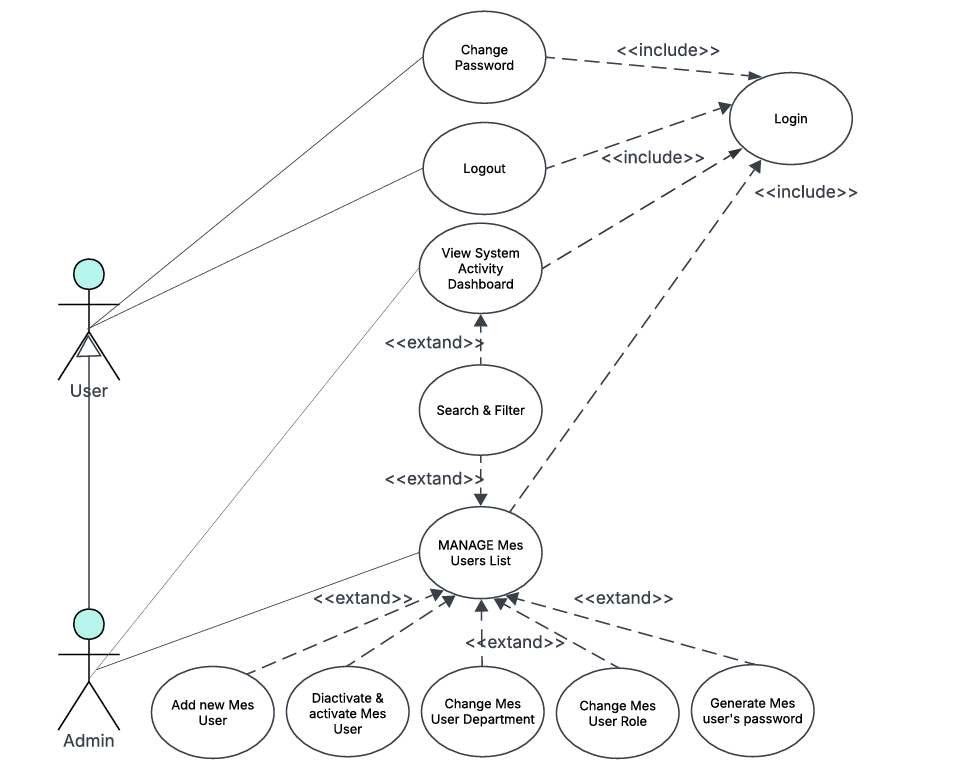
\includegraphics[width=\linewidth,keepaspectratio]{./media/MES_Sprint-1-Repport/diagrams/useCase/sprint1.png}
	\caption{UML Use Case Diagram.}
	\label{fig:s1-use-case-diagram}
\end{figure}

\Needspace{10\baselineskip}
\subsection{Textual Use Case Description}

\begin{longtable}{@{} P{0.22\linewidth} P{0.78\linewidth} @{}}
	
	\toprule
	\endfirsthead
	
	\midrule
	\endhead
	
	\multicolumn{2}{r}{\small Continued on next page}\\
	\endfoot
	
	\endlastfoot
	
	\textbf{Use Case Name}  & Login                                                                \\
	\midrule
	\textbf{Primary Actors} & \userrole{Operator}, \userrole{Supervisor}, \userrole{Administrator} \\
	\midrule
	\textbf{Preconditions}  &                                                                      
	\begin{itemize}[noitemsep, topsep=0pt, partopsep=0pt, leftmargin=*]
	\item The user account exists in the \techname{ERP} system.
	\item The user has an assigned role and department.
	\item The account must have a password (there is a possibility that
	there is an account without a password).
	\item The user account is active.
	\end{itemize} \\
	\midrule
	
	\textbf{Postconditions} &                                                                      
	\begin{itemize}[noitemsep, topsep=0pt, partopsep=0pt, leftmargin=*]
	\item If the credentials are valid, the user is successfully authenticated.
	\item A session token is generated and stored securely.
	\item The user is redirected to the appropriate dashboard based on their
	role (\userrole{Admin} or MES interface).
	\item If the \domainterm{need change password} flag is set to true, they
	are redirected to the \uilabel{Change Password} page.
	\item If the credentials are invalid, access is denied and an error
	message is displayed.
	\end{itemize} \\
	\midrule
	
	\textbf{Main Scenario}  &                                                                      
	\begin{enumerate}[noitemsep, topsep=0pt, partopsep=0pt, leftmargin=*]
	\item The user launches the application.
	\item The system displays the \uilabel{login screen}.
	\item The user enters \uilabel{Auth ID} and \uilabel{password}.
	\item The system automatically detects the device ID.
	\item The user clicks the \uilabel{Login} button.
	\item The system validates the credentials against the \techname{ERP} database.
	\item The system generates a secure session token.
	\item The system checks the user role.
	\item The system redirects the user to the appropriate dashboard
	(\userrole{Admin} or MES).
	\end{enumerate} \\
	\midrule
	\noalign{\vskip 4pt}
	\caption{Textual Use Case Description --- Login}
	\label{tab:s1-use-case-login}
	
\end{longtable}

\subsection{Sequence Diagrams}

The following sequence diagrams illustrate the communication flow between the
\techname{Flutter} frontend, the \techname{Business Central} OData layer, and
the \techname{AL} business logic for each authentication flow.
 
Figure~\ref{fig:s1-seq-login} depicts the login flow, in which the user submits
credentials, the \techname{AL} layer validates them against the
\techname{Business Central} user store, and the application either returns a
structured error or issues a session token and redirects the user to the
appropriate page based on their role and password-change flag.
\begin{figure}[H]
	\centering
	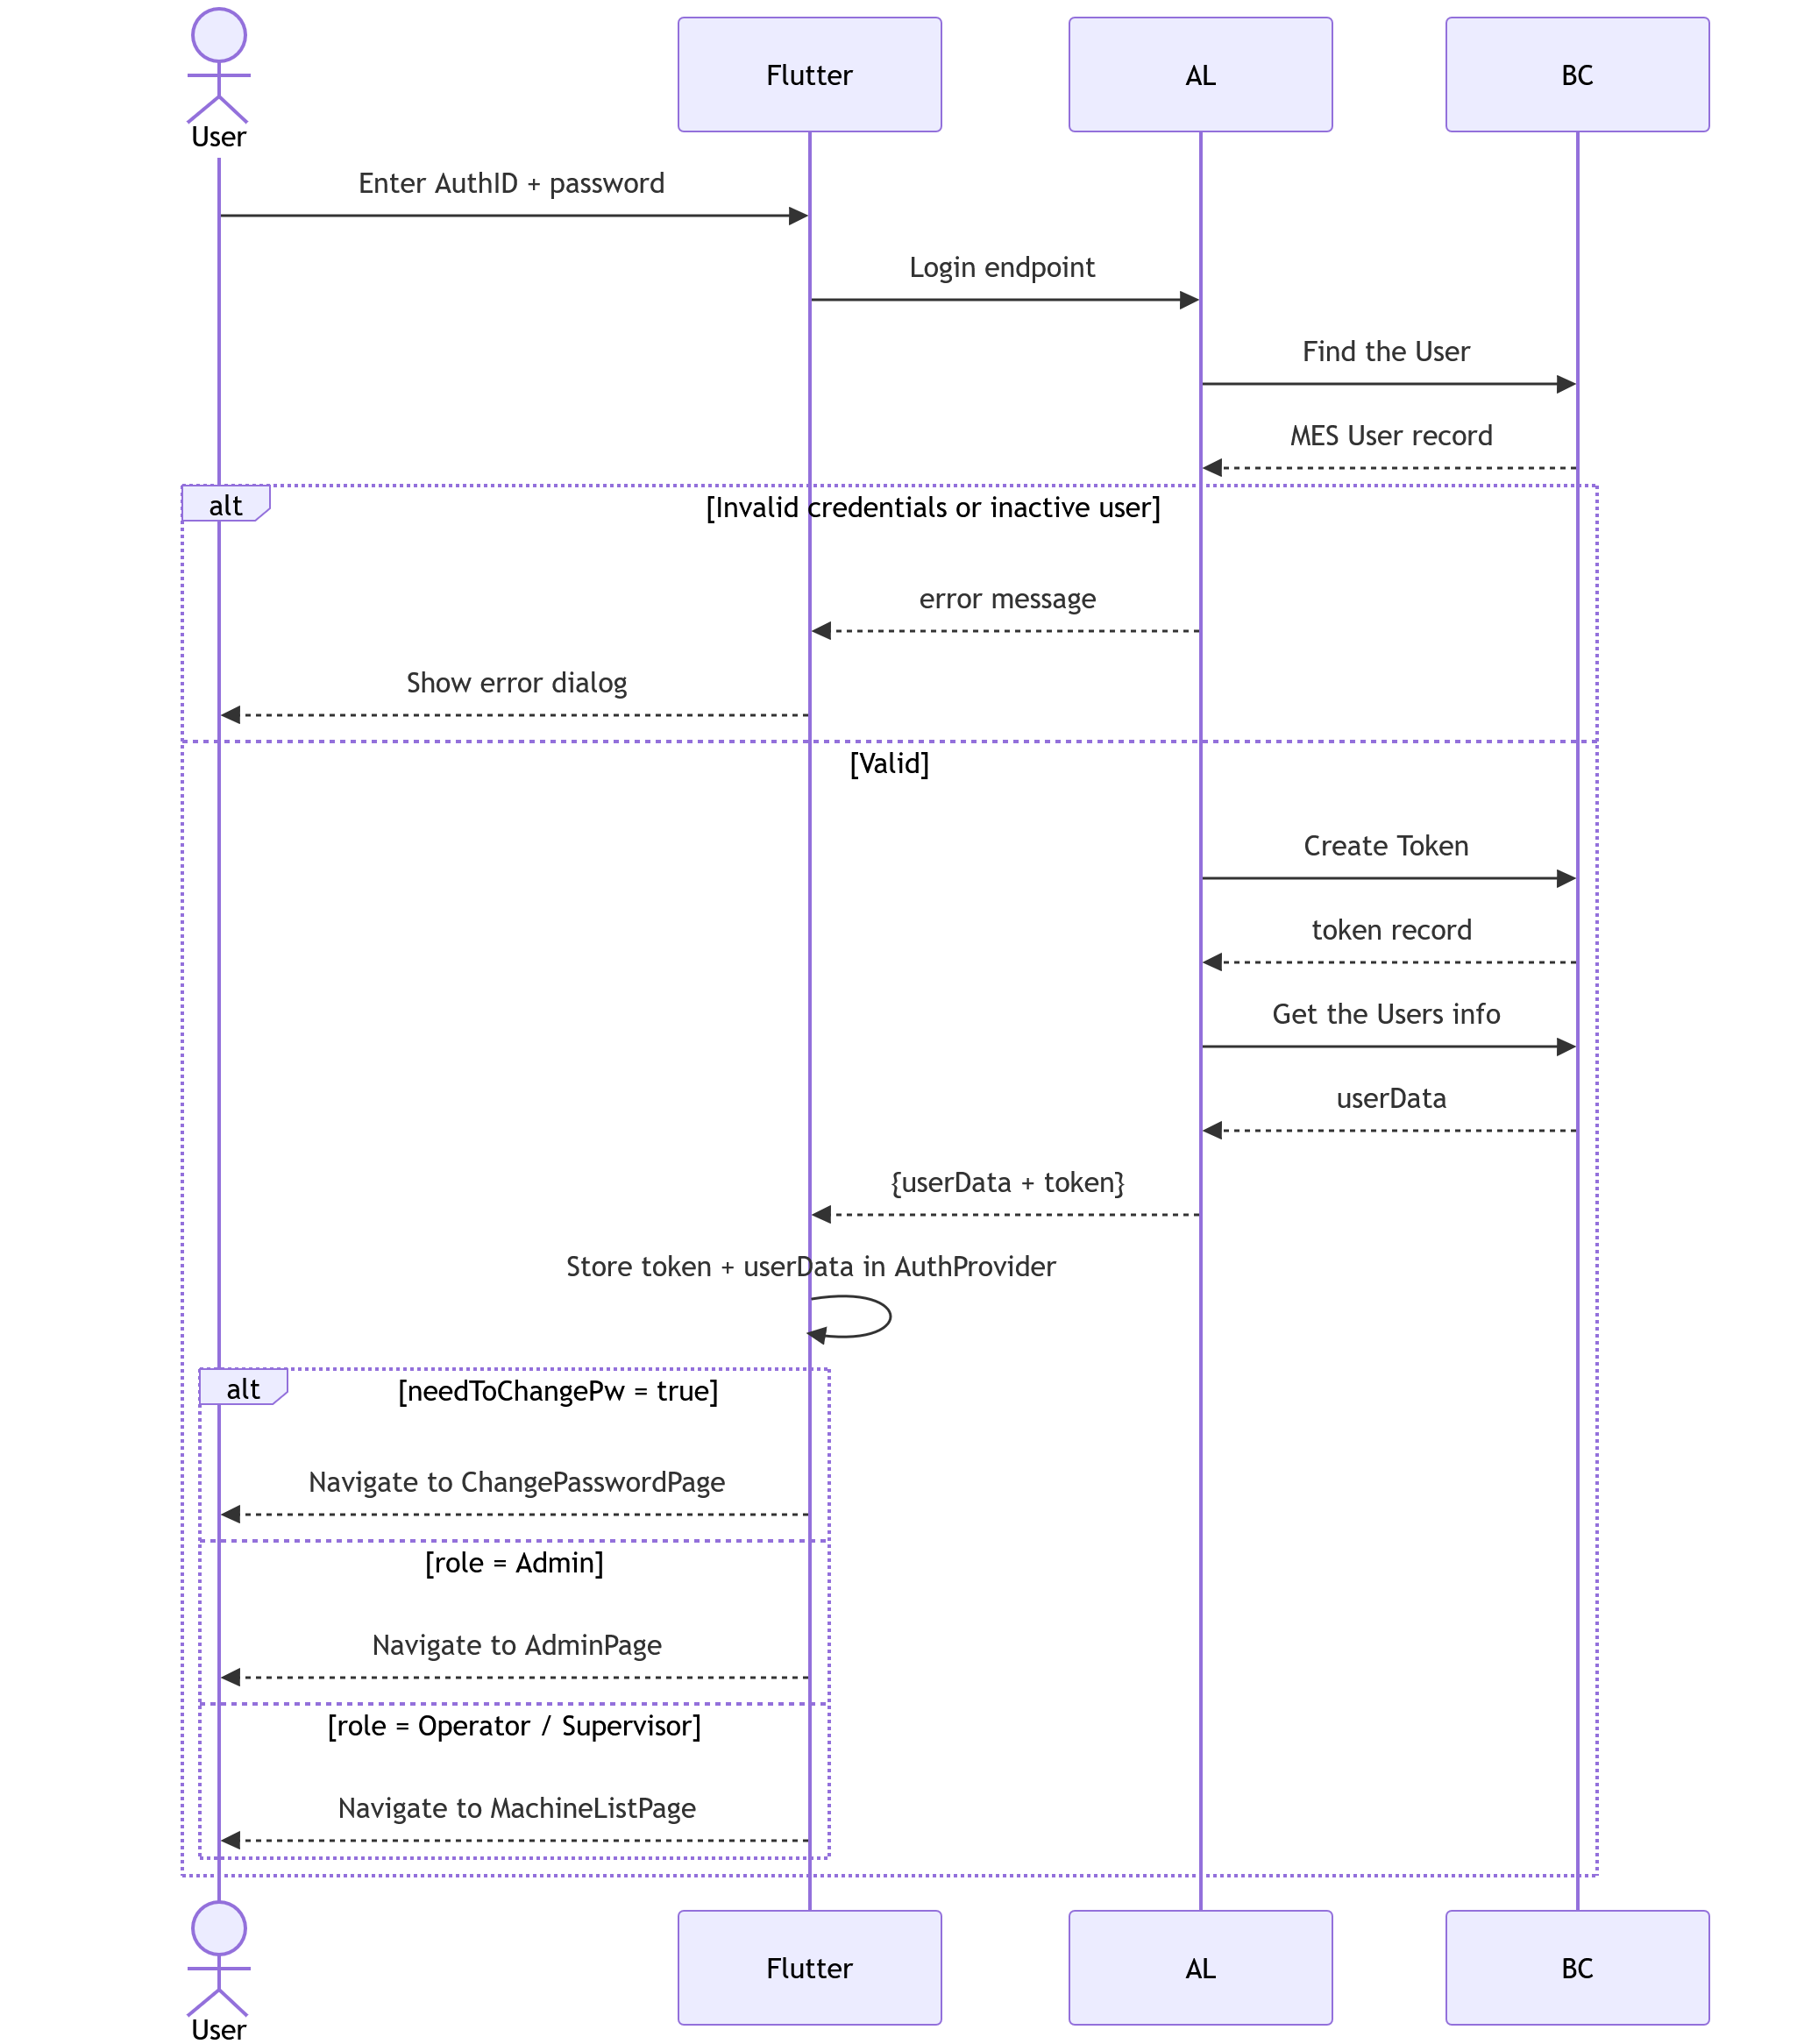
\includegraphics[width=\linewidth,height=0.82\textheight,keepaspectratio]{./media/MES_Sprint-1-Repport/diagrams/sequence/login.png}%
	\caption{SD-01: Login.}%
	\label{fig:s1-seq-login}%
\end{figure}%

%=====SD-01==========================================================
% sequenceDiagram
%    actor User
%    participant Flutter
%    participant AL
%    participant BC

%    User->>Flutter: Enter AuthID + password
%    Flutter->>AL: Login endpoint
%    AL->>BC: Find the User 
%    BC-->>AL: MES User record
%    alt Invalid credentials or inactive user
%        AL-->>Flutter: error message
%        Flutter-->>User: Show error dialog
%    else Valid
%        AL->>BC: Create Token
%        BC-->>AL: token record
%        AL->>BC: Get the Users info
%        BC-->>AL: userData
%        AL-->>Flutter: {userData + token}
%        Flutter->>Flutter: Store token + userData in AuthProvider
%        alt needToChangePw = true
%            Flutter-->>User: Navigate to ChangePasswordPage
%        else role = Admin
%            Flutter-->>User: Navigate to AdminPage
%        else role = Operator / Supervisor
%            Flutter-->>User: Navigate to MachineListPage
%        end
%    end
%====================================================================

Figure~\ref{fig:s1-seq-Token-Validation} presents the token validation flow,
which is invoked by the \techname{AL} backend before processing any
authenticated request. The backend retrieves the token record from
\techname{Business Central}, verifies its validity and expiry, confirms
that the associated user account is still active, and either updates the
\texttt{LastSeenAt} timestamp or returns an error that forces the
\techname{Flutter} client to redirect the user to the login page.
 

\begin{figure}[H]
	\centering
	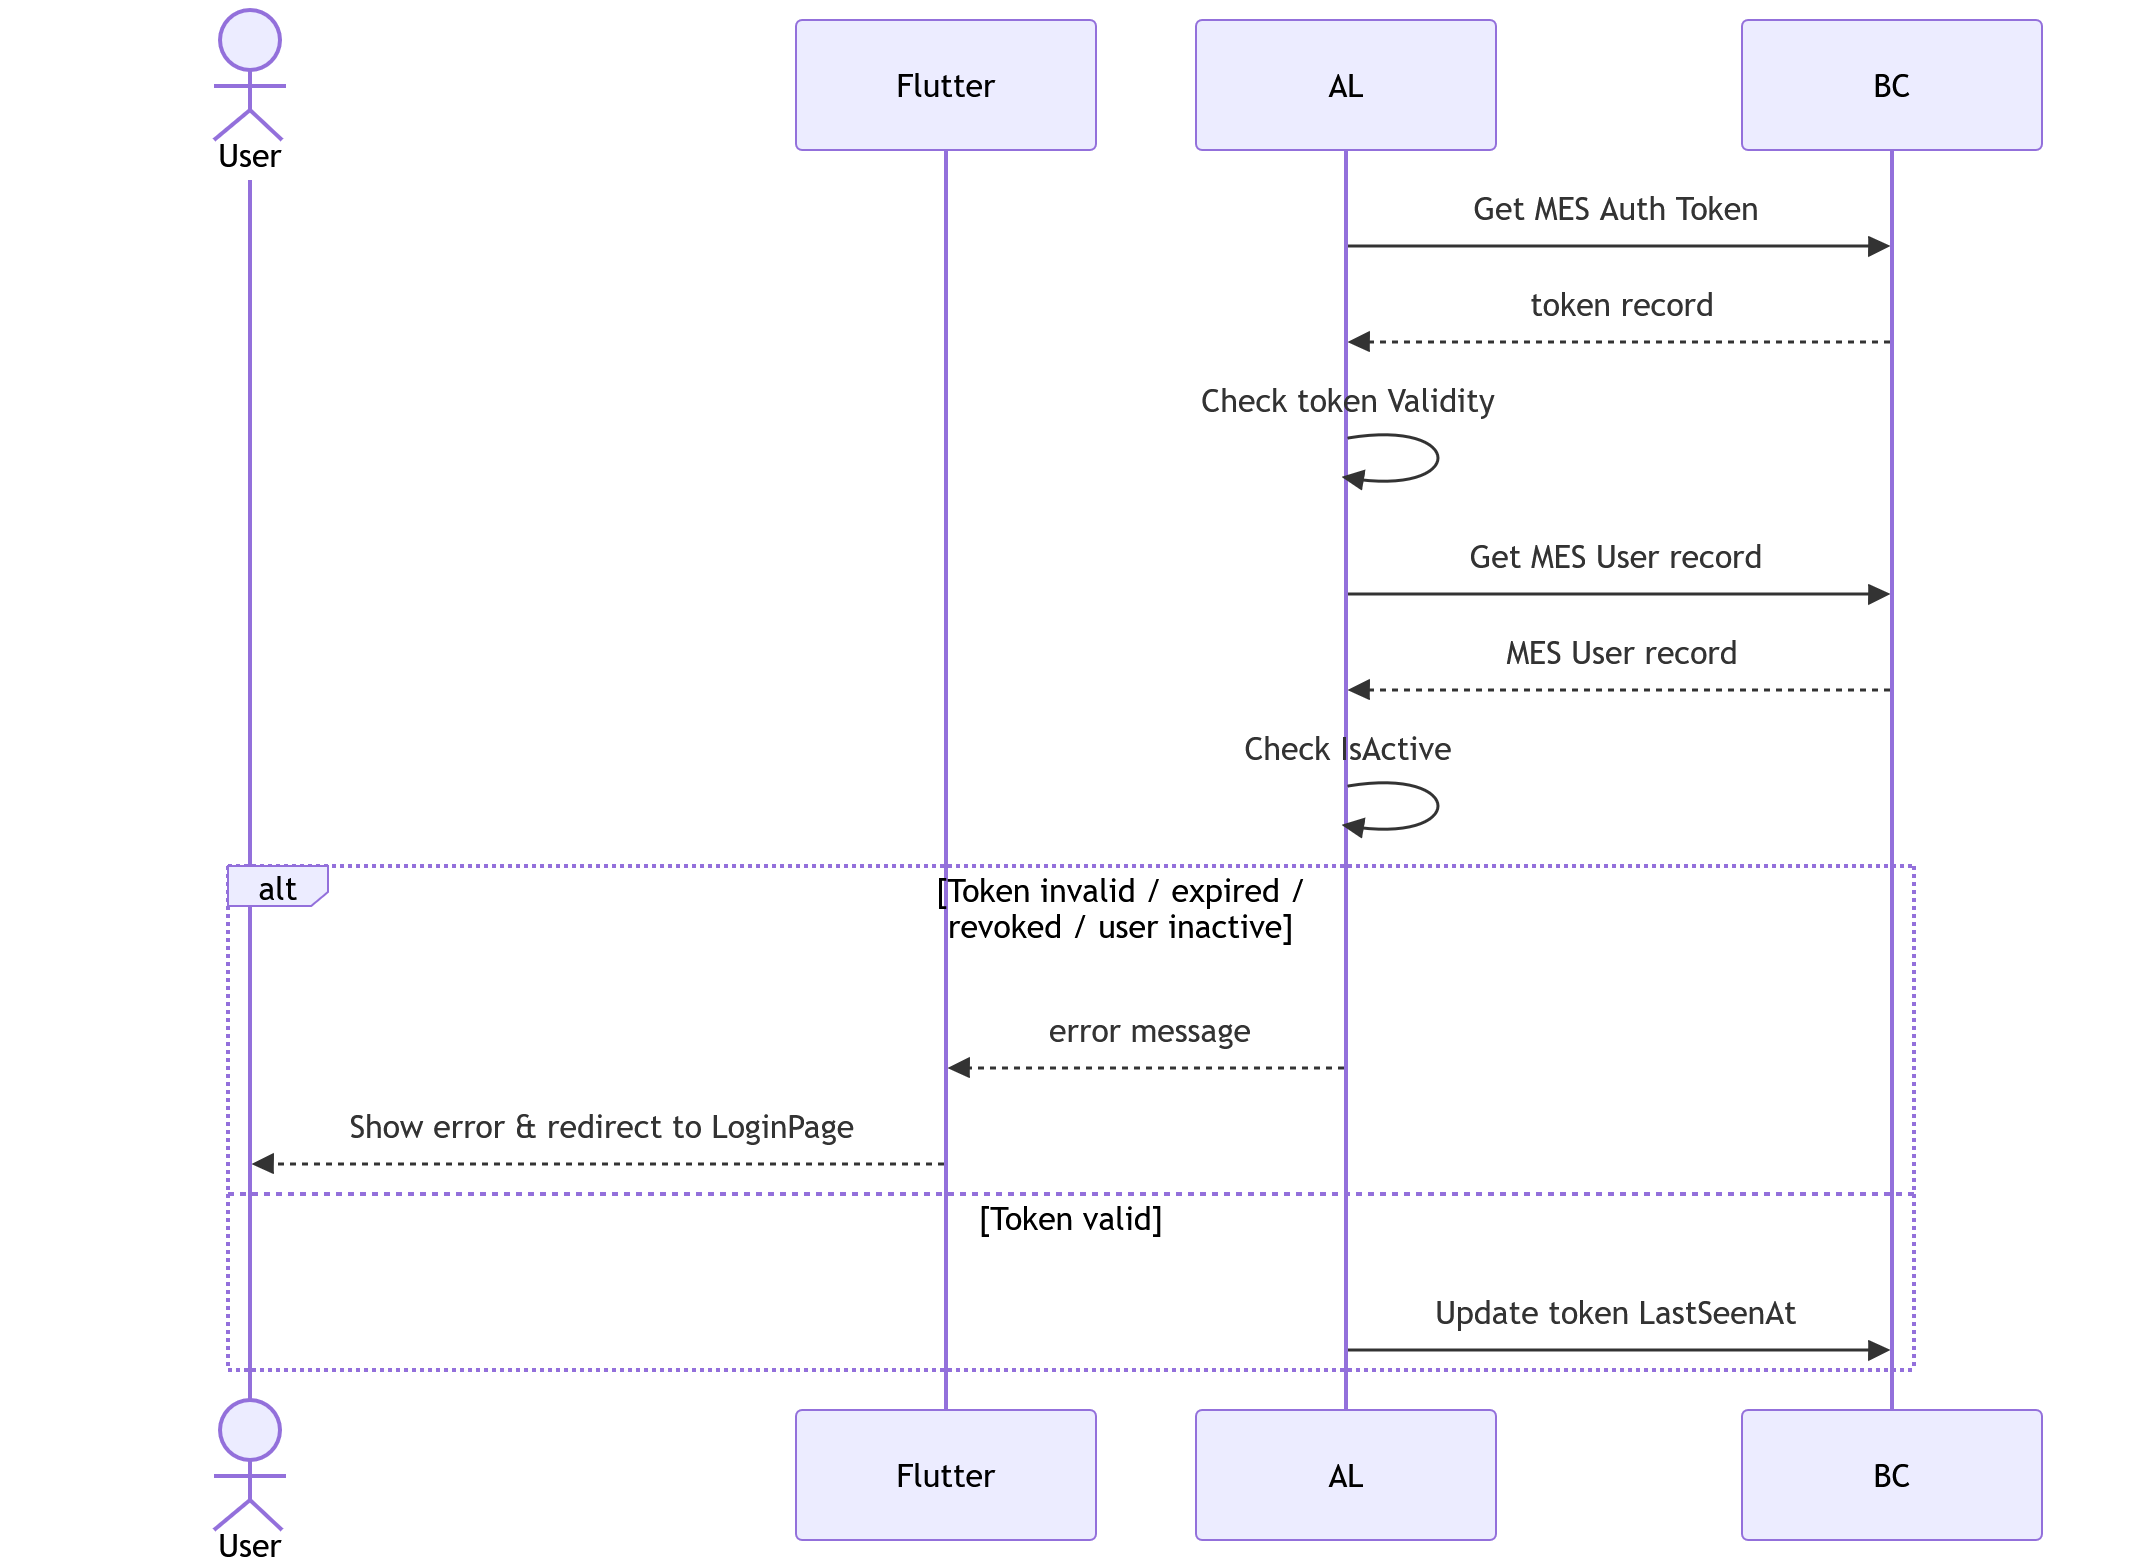
\includegraphics[width=\linewidth,height=0.82\textheight,keepaspectratio]{./media/MES_Sprint-1-Repport/diagrams/sequence/token-validation.png}%
	\caption{SD-02: Token Validation.}%
	\label{fig:s1-seq-Token-Validation}%
\end{figure}%

%======SD-02=========================================================
% sequenceDiagram
%     actor User
%     participant Flutter
%     participant AL
%     participant BC

%     AL->>BC: Get MES Auth Token
%     BC-->>AL: token record
%     AL->>AL: Check token Validity
%     AL->>BC: Get MES User record
%     BC-->>AL: MES User record
%     AL->>AL: Check IsActive
%     alt Token invalid / expired / revoked / user inactive
%         AL-->>Flutter: error message
%         Flutter-->>User: Show error & redirect to LoginPage
%     else Token valid
%         AL->>BC: Update token LastSeenAt
%     end
%====================================================================

Figure~\ref{fig:s1-seq-logout} illustrates the logout flow, in which the
\techname{Flutter} client sends a logout request, the \techname{AL} layer
retrieves and revokes the current session token in \techname{Business Central},
and the client clears its local \techname{AuthProvider} state before
navigating back to the login page.

\begin{figure}[H]
	\centering
	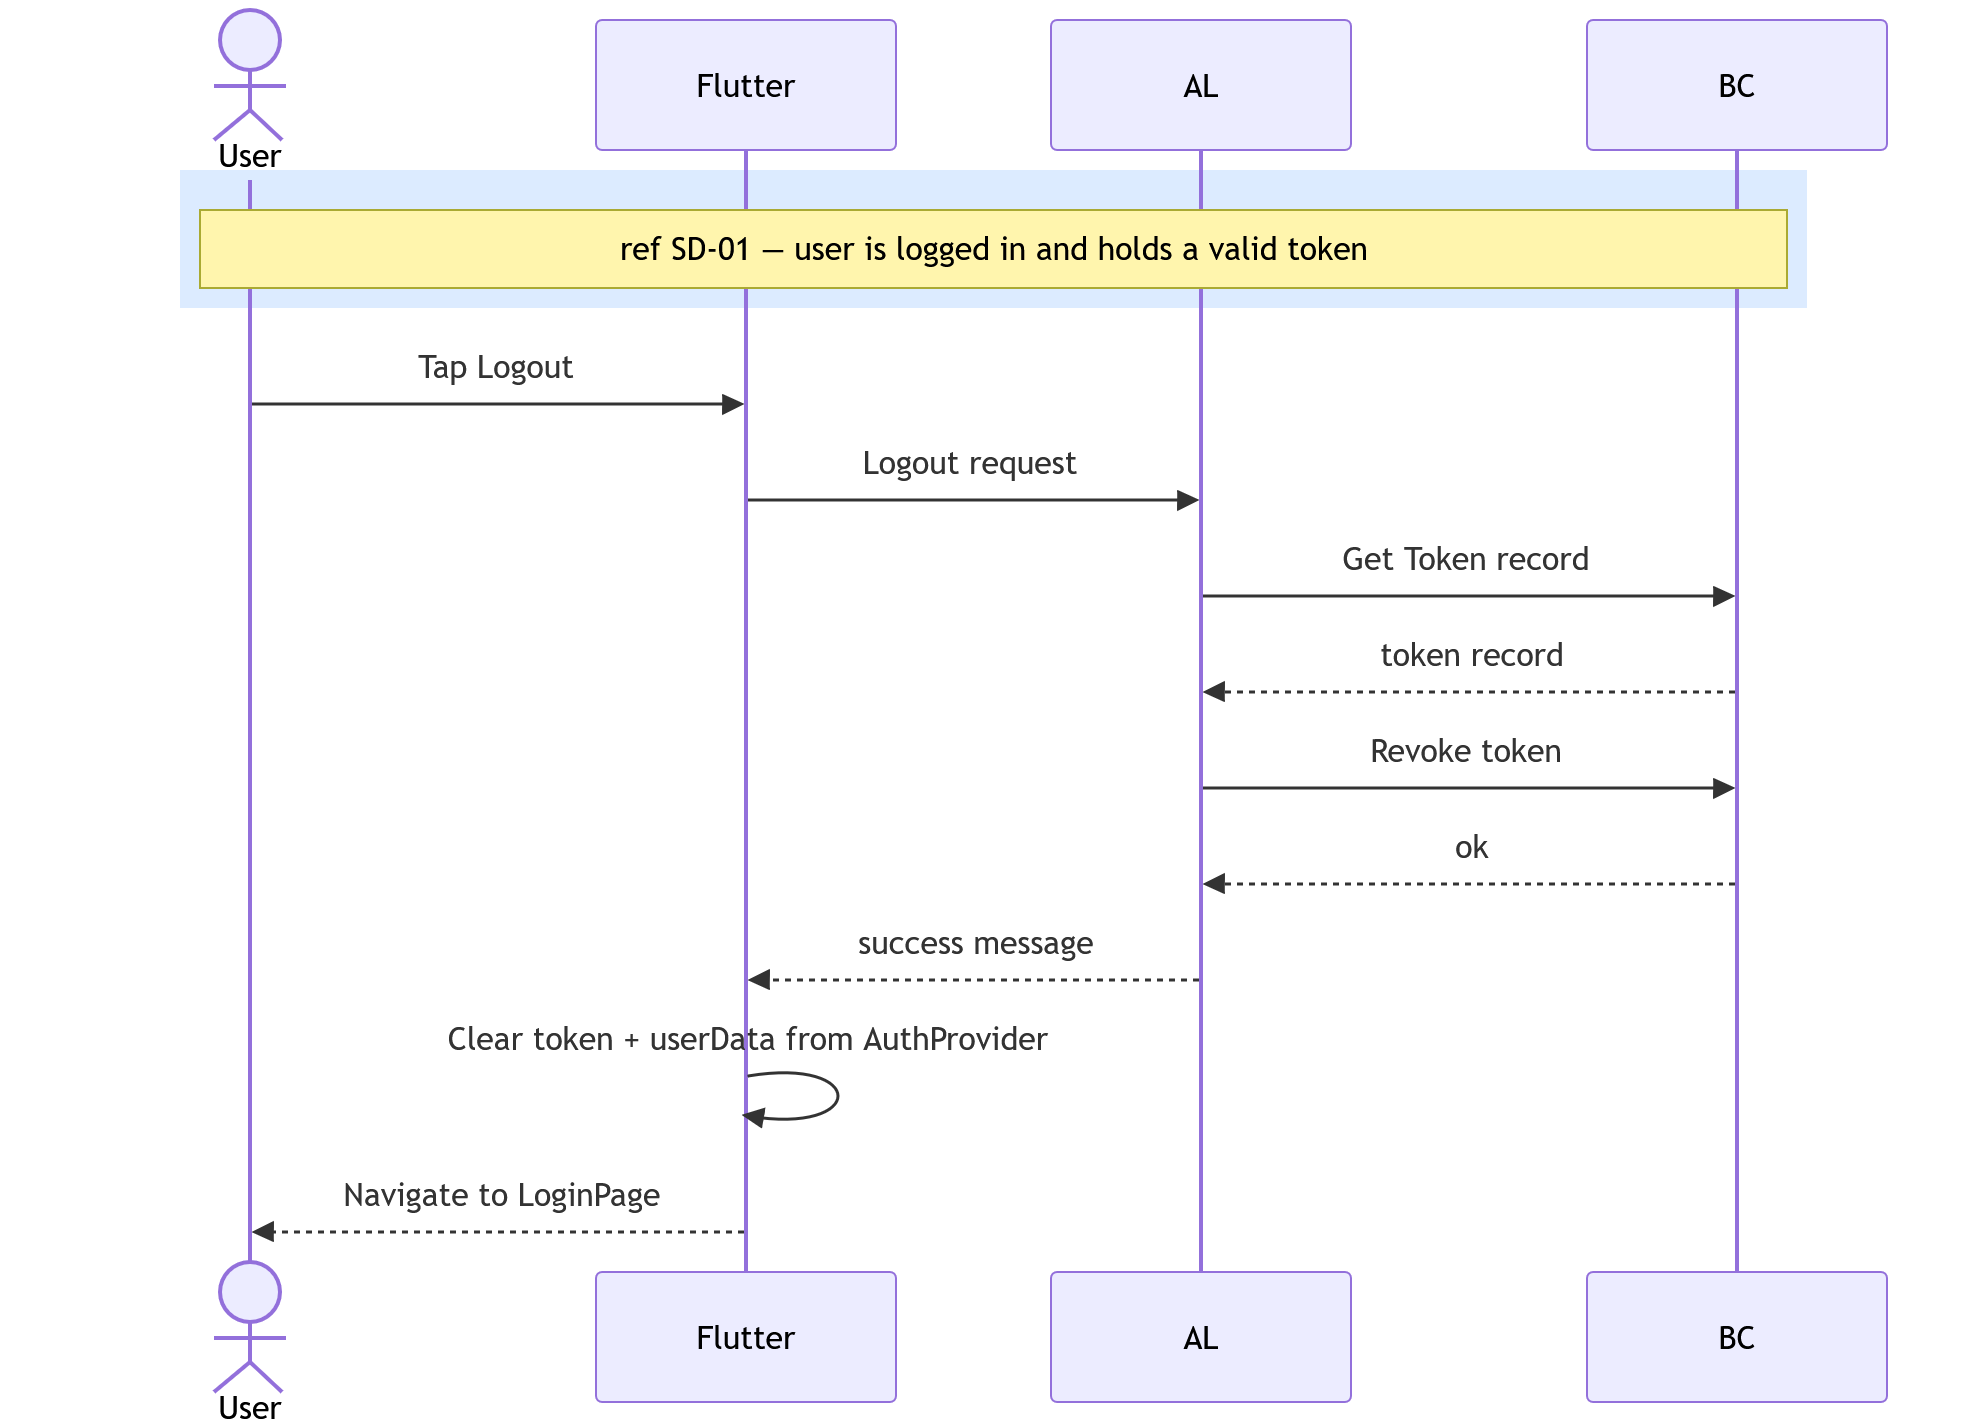
\includegraphics[width=\linewidth,height=0.82\textheight,keepaspectratio]{./media/MES_Sprint-1-Repport/diagrams/sequence/logout.png}%
	\caption{SD-03: Logout}%
	\label{fig:s1-seq-logout}%
\end{figure}%

%======SD-03=========================================================
% sequenceDiagram
%     actor User
%     participant Flutter
%     participant AL
%     participant BC

%     rect rgb(220,235,255)
%         Note over User,BC: ref SD-01 — user is logged in and holds a valid token
%     end

%     User->>Flutter: Tap Logout
%     Flutter->>AL: Logout request
%     AL->>BC: Get Token record
%     BC-->>AL: token record
%     AL->>BC: Revoke token
%     BC-->>AL: ok
%     AL-->>Flutter: success message
%     Flutter->>Flutter: Clear token + userData from AuthProvider
%     Flutter-->>User: Navigate to LoginPage
%====================================================================

Figure~\ref{fig:s1-seq-ChangePw} describes the change-password flow. The
\techname{Flutter} client first validates locally that the two password
fields match and satisfy the strength rules, then forwards the request to
the \techname{AL} layer, which re-validates the token (SD-02), verifies
the current password hash, checks the new password strength, and — on
success — updates the credential record in \techname{Business Central}
and revokes all existing tokens for the account.

\begin{figure}[H]
	\centering
	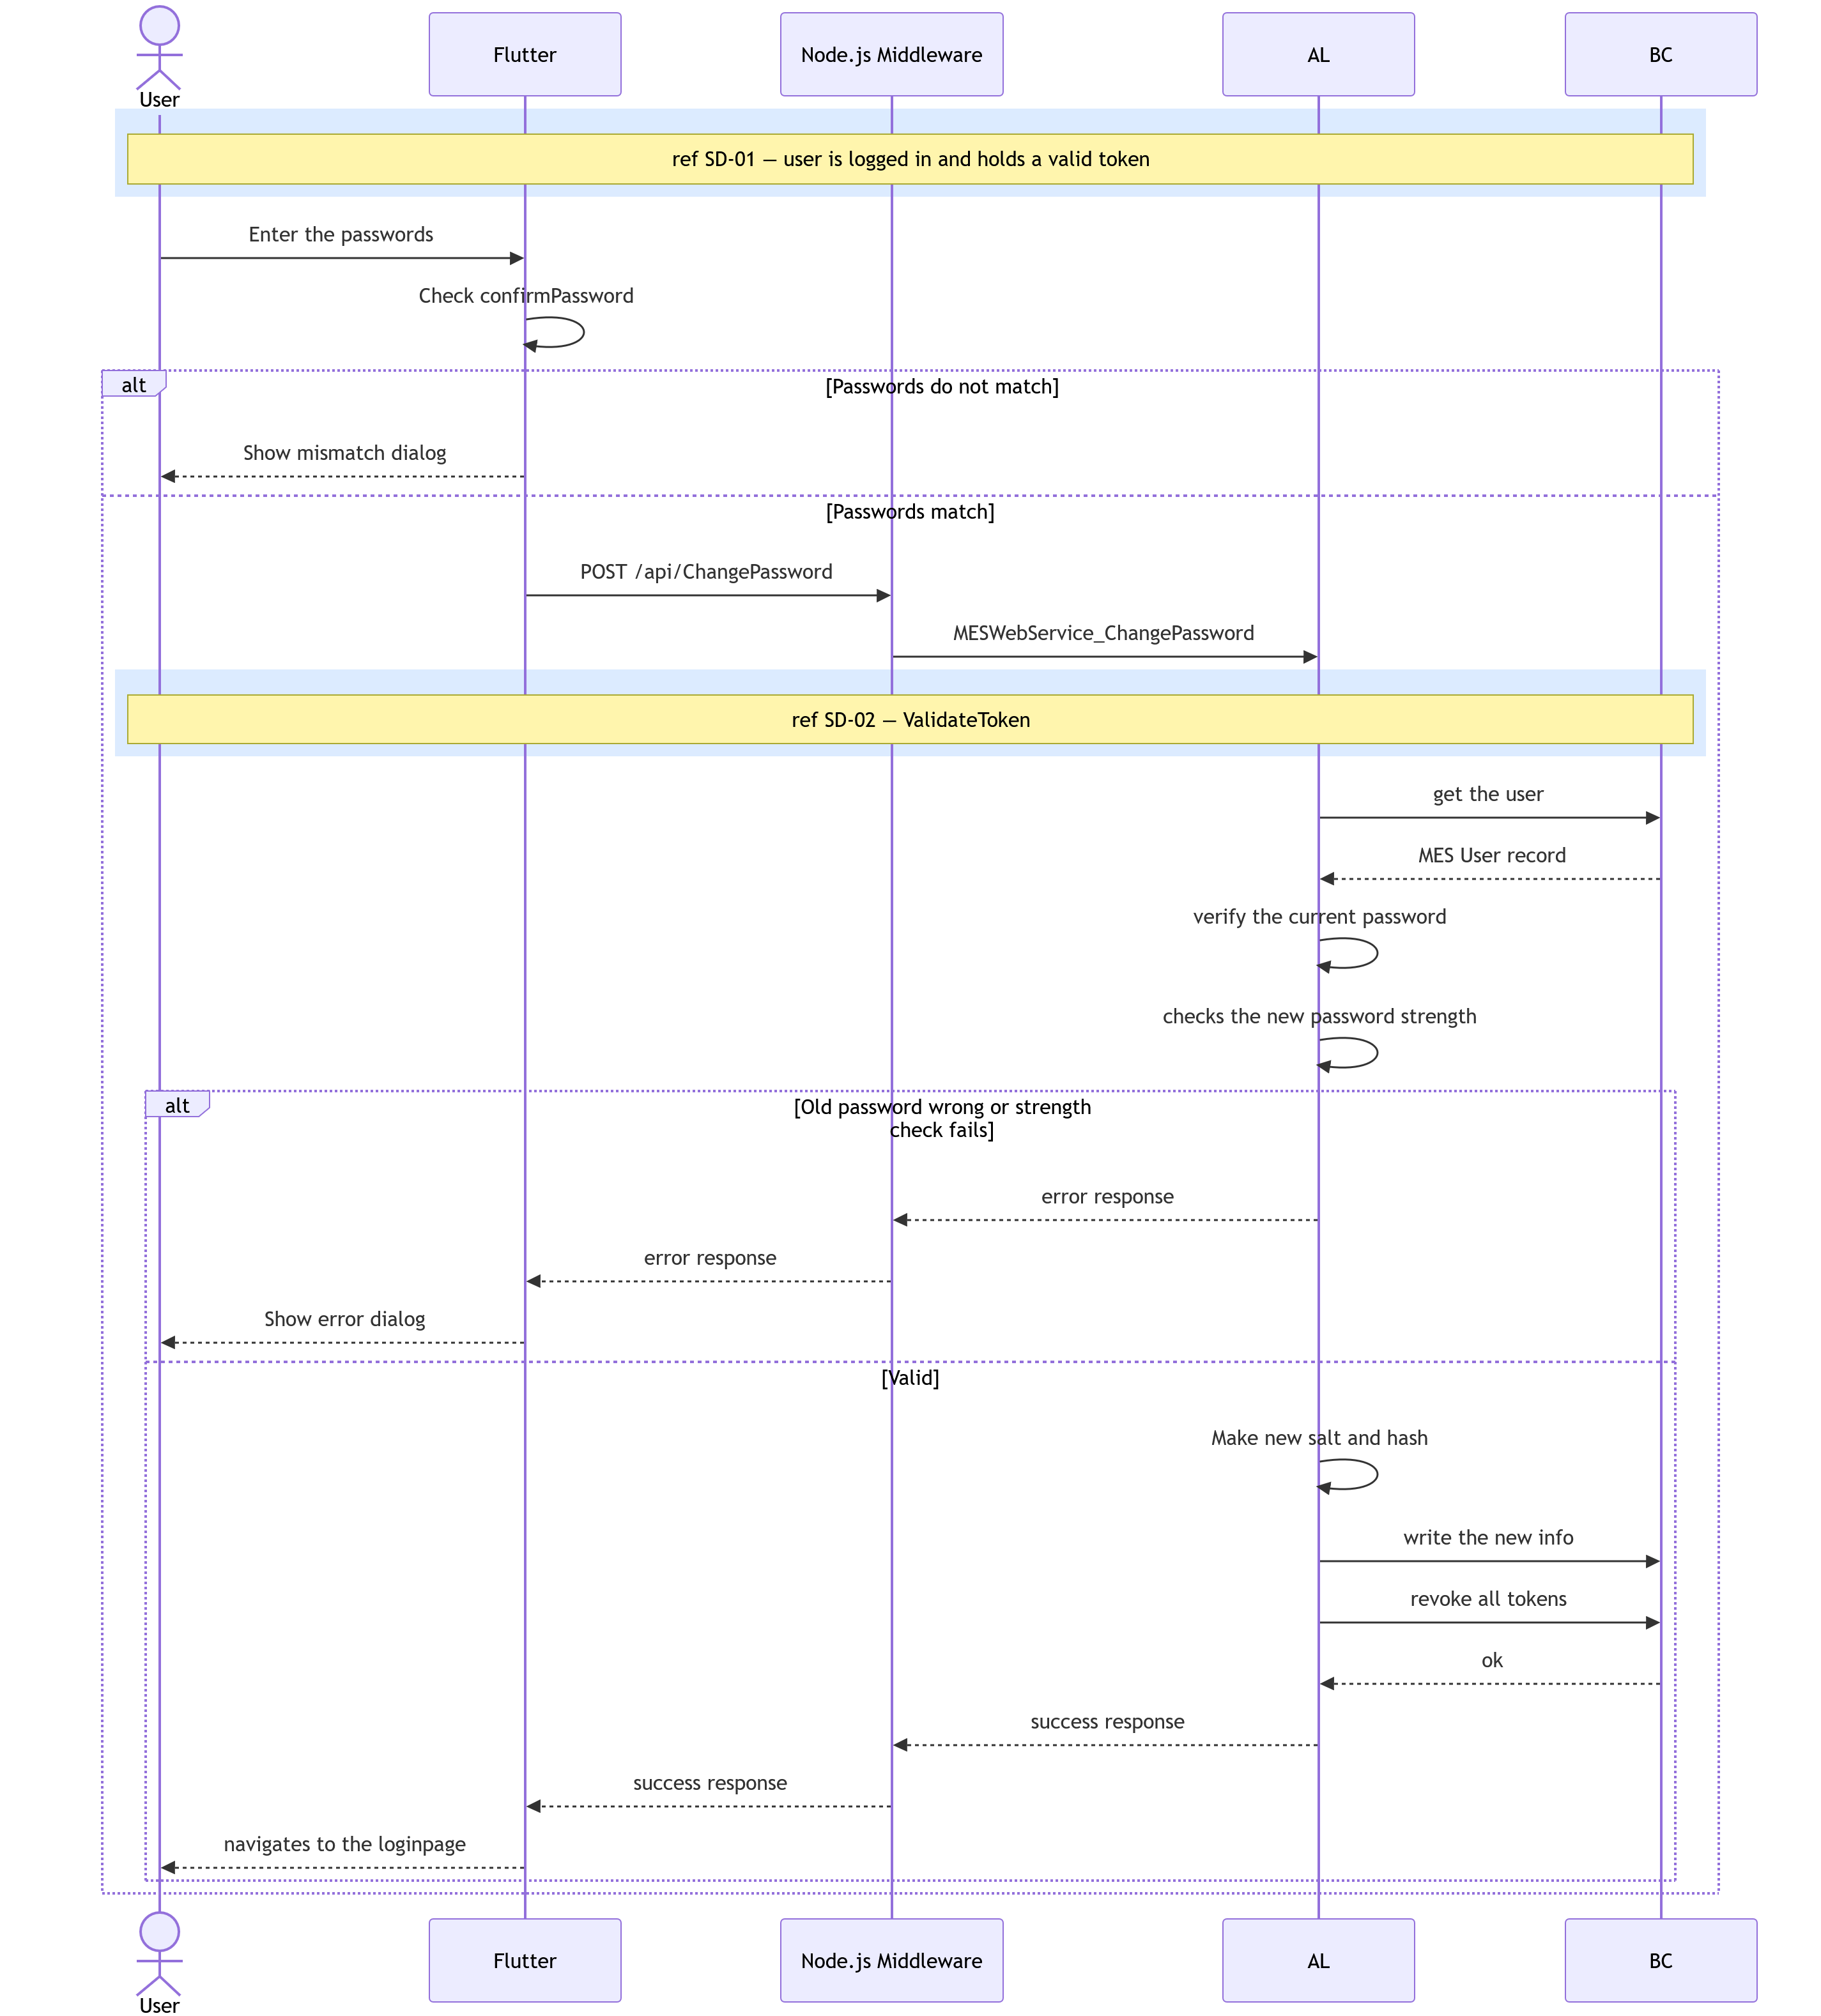
\includegraphics[width=\linewidth,height=0.82\textheight,keepaspectratio]{./media/MES_Sprint-1-Repport/diagrams/sequence/change-password.png}%
	\caption{SD-03: Change Password}%
	\label{fig:s1-seq-ChangePw}%
\end{figure}%


%======SD-04=========================================================
% sequenceDiagram
%     actor User
%     participant Flutter
%     participant AL
%     participant BC

%     rect rgb(220,235,255)
%         Note over User,BC: ref SD-01 — user is logged in and holds a valid token
%     end

%     User->>Flutter: Enter current password + new password
%     Flutter->>Flutter: Validate passwords match and meet strength rules
%     Flutter->>AL: ChangePassword request

%     rect rgb(220,235,255)
%         Note over User,BC: ref SD-02 — AL validates token before proceeding
%     end

%     AL->>BC: Get MES User (from token)
%     BC-->>AL: MES User record (storedHash, salt)
%     AL->>AL: check old password
%     AL->>AL: IsPasswordStrong(newPw)
%     alt Validation failed
%         AL-->>Flutter: error message
%         Flutter-->>User: Show error dialog
%     else Valid
%         AL->>BC: Update MES User with new password
%         AL->>BC: Revoke all tokens of the user
%         BC-->>AL: ok
%         AL-->>Flutter: success message
%         Flutter->>Flutter: Update AuthProvider 
%         Flutter-->>User: Navigate to AdminPage / MachineListPage
%     end
%====================================================================

Figures~\ref{fig:s1-seq-AdminCreateUser} through~\ref{fig:s1-seq-AdminToggleActive}
cover the four administrator user-management operations. All four follow the
same pattern: the \techname{Flutter} client sends an admin-scoped request,
the \techname{AL} layer validates the token and confirms that the caller
holds the \userrole{Admin} role (SD-02), executes the requested
\techname{Business Central} write operations, and triggers a reactive refresh
so that the updated user list is reflected immediately in the UI.
 
Figure~\ref{fig:s1-seq-AdminCreateUser} shows the user creation flow, in which
the \techname{AL} layer inserts a new \domainterm{MES User} record with
\texttt{IsActive} and \texttt{NeedToChangePw} set to \texttt{true}, then
iterates over the supplied work-centre list to create the corresponding
assignment records.

\begin{figure}[H]
	\centering
	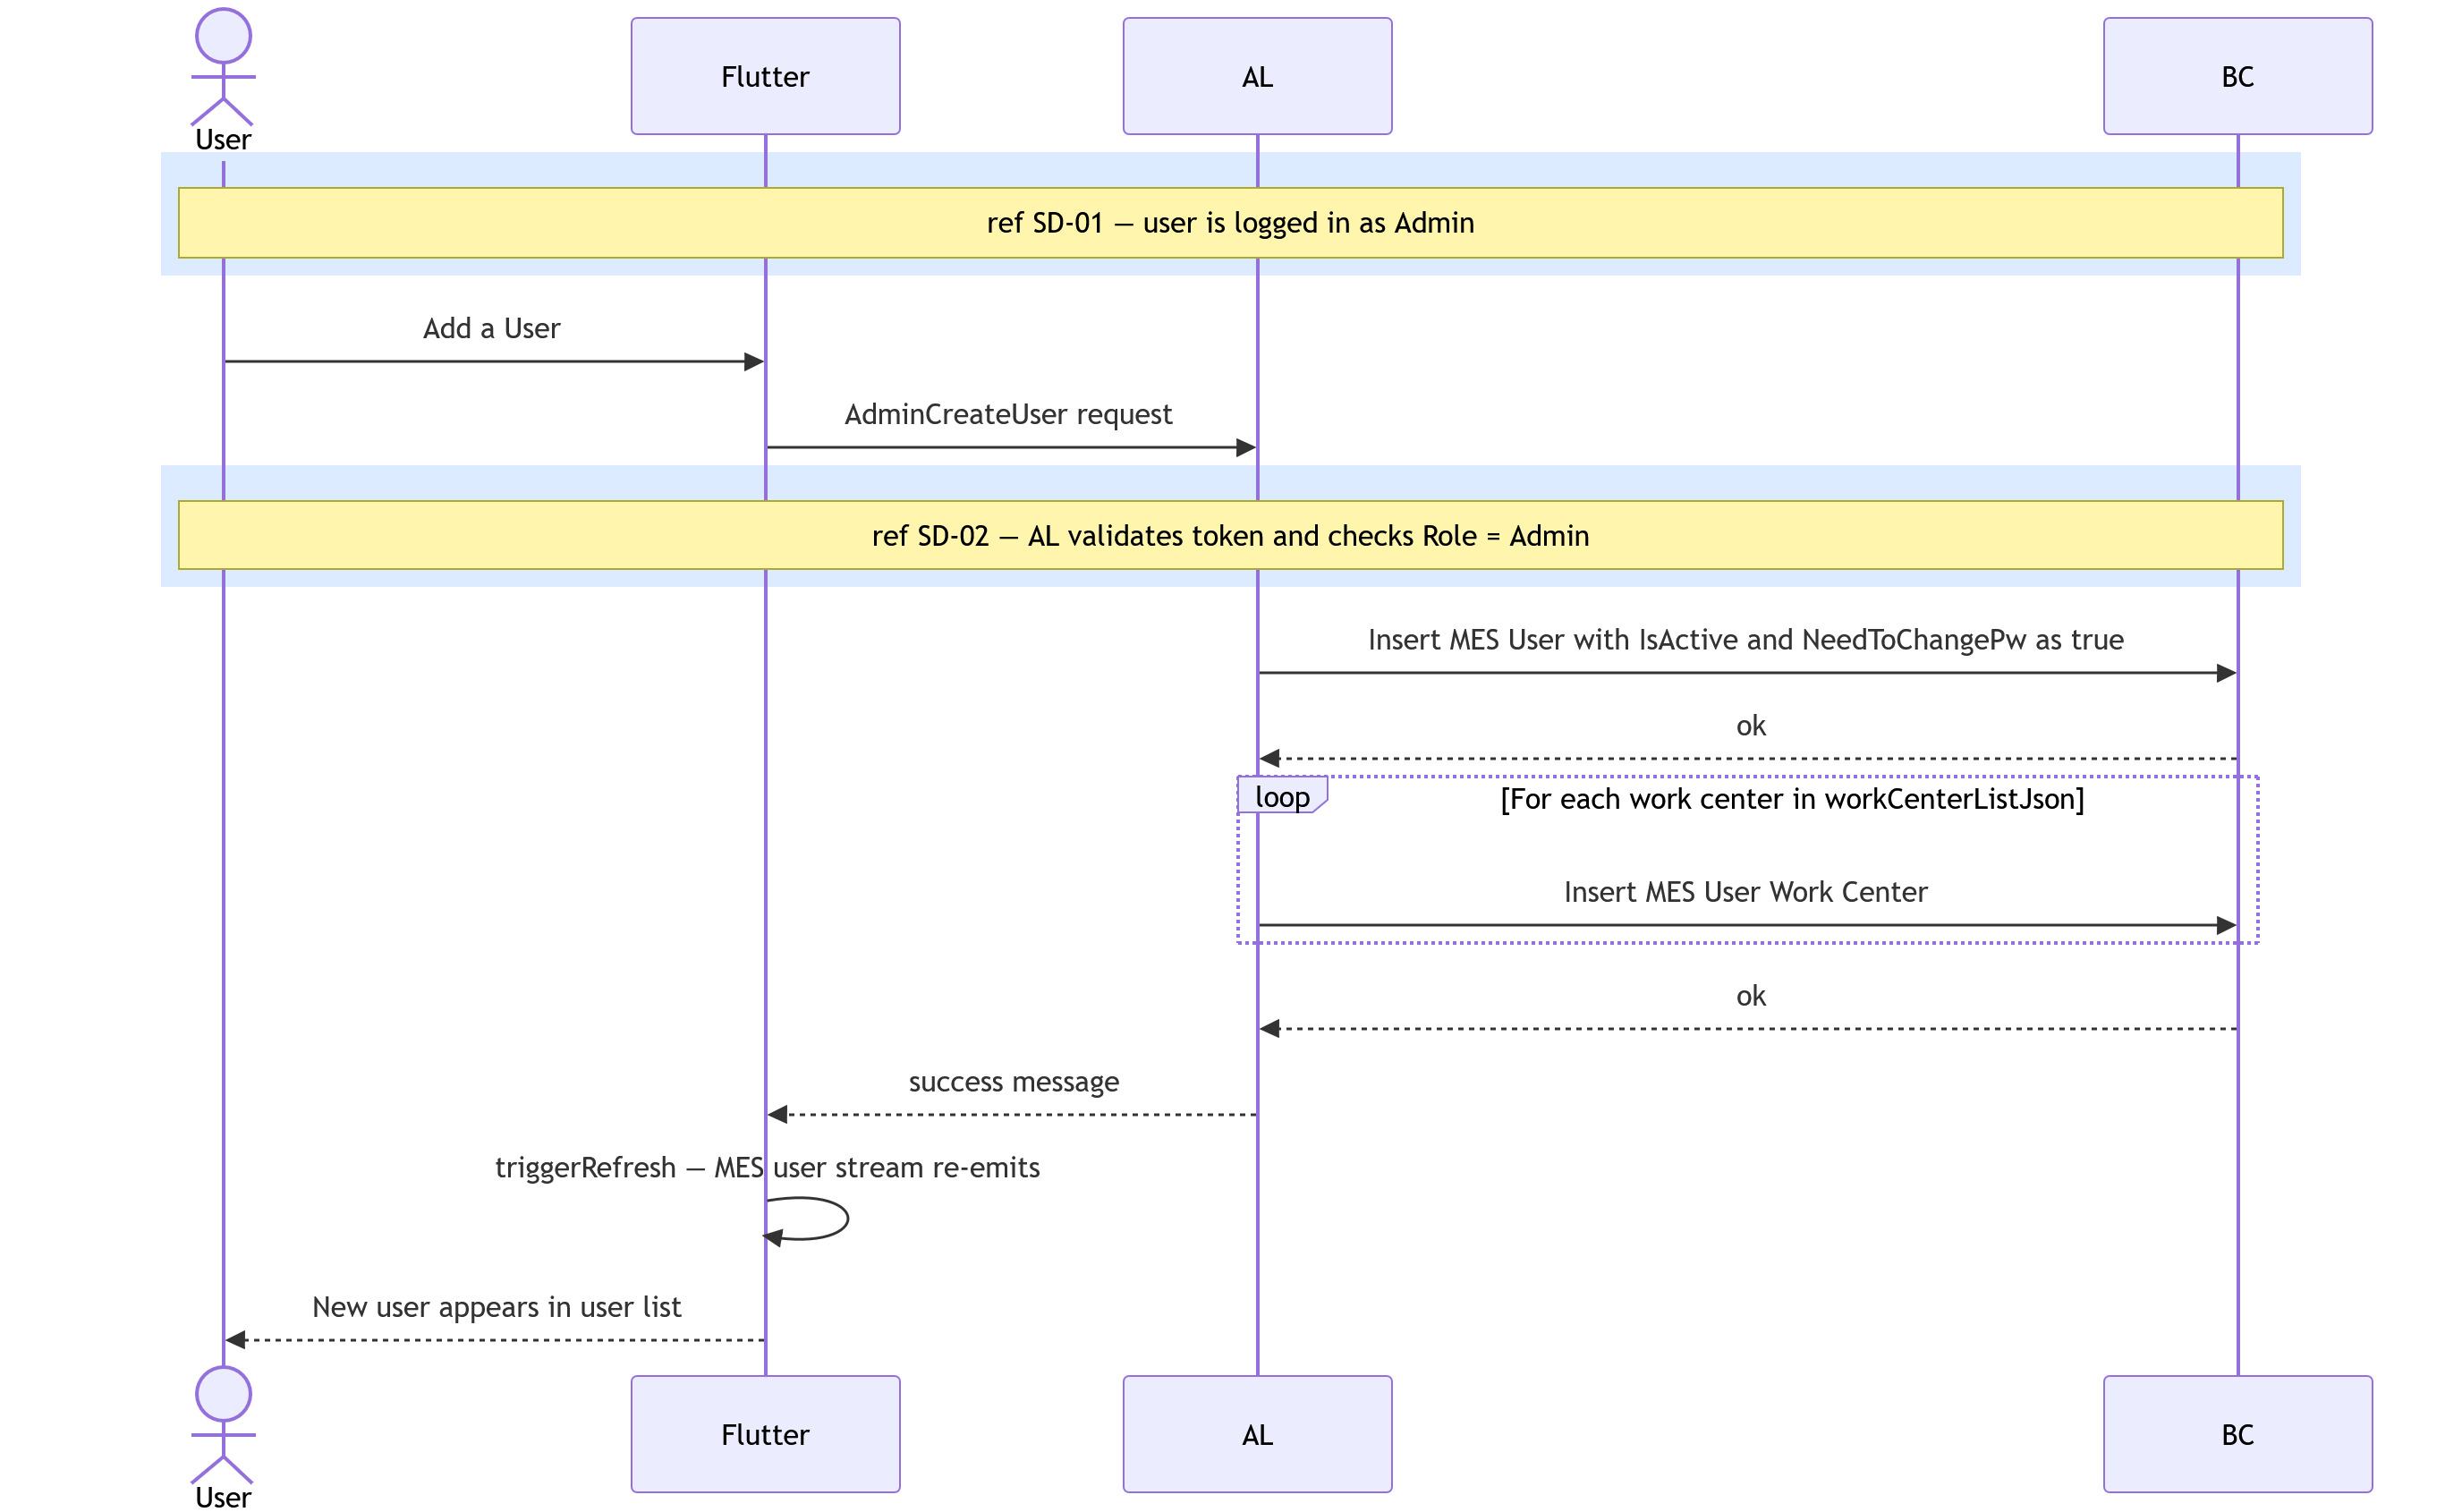
\includegraphics[width=\linewidth,height=0.82\textheight,keepaspectratio]{./media/MES_Sprint-1-Repport/diagrams/sequence/admin-create-user.png}%
	\caption{SD-05: Admin - Create User.}%
	\label{fig:s1-seq-AdminCreateUser}%
\end{figure}%

%=====SD:05==========================================================
% sequenceDiagram
%     actor User
%     participant Flutter
%     participant AL
%     participant BC

%     rect rgb(220,235,255)
%         Note over User,BC: ref SD-01 — user is logged in as Admin
%     end

%     User->>Flutter: Add a User
%     Flutter->>AL: AdminCreateUser request

%     rect rgb(220,235,255)
%         Note over User,BC: ref SD-02 — AL validates token and checks Role = Admin
%     end

%     AL->>BC: Insert MES User with IsActive and NeedToChangePw as true
%     BC-->>AL: ok
%     loop For each work center in workCenterListJson
%         AL->>BC: Insert MES User Work Center
%     end
%     BC-->>AL: ok
%     AL-->>Flutter: success message
%     Flutter->>Flutter: triggerRefresh — MES user stream re-emits
%     Flutter-->>User: New user appears in user list
%====================================================================

Figure~\ref{fig:s1-seq-AdminSetPw} depicts the admin set-password flow. The
administrator generates a temporary credential, the \techname{AL} layer marks
the target account as requiring a password change on next login, revokes all
active tokens for that account, and returns the new credential to the
\techname{Flutter} client as copyable text.

\begin{figure}[H]
	\centering
	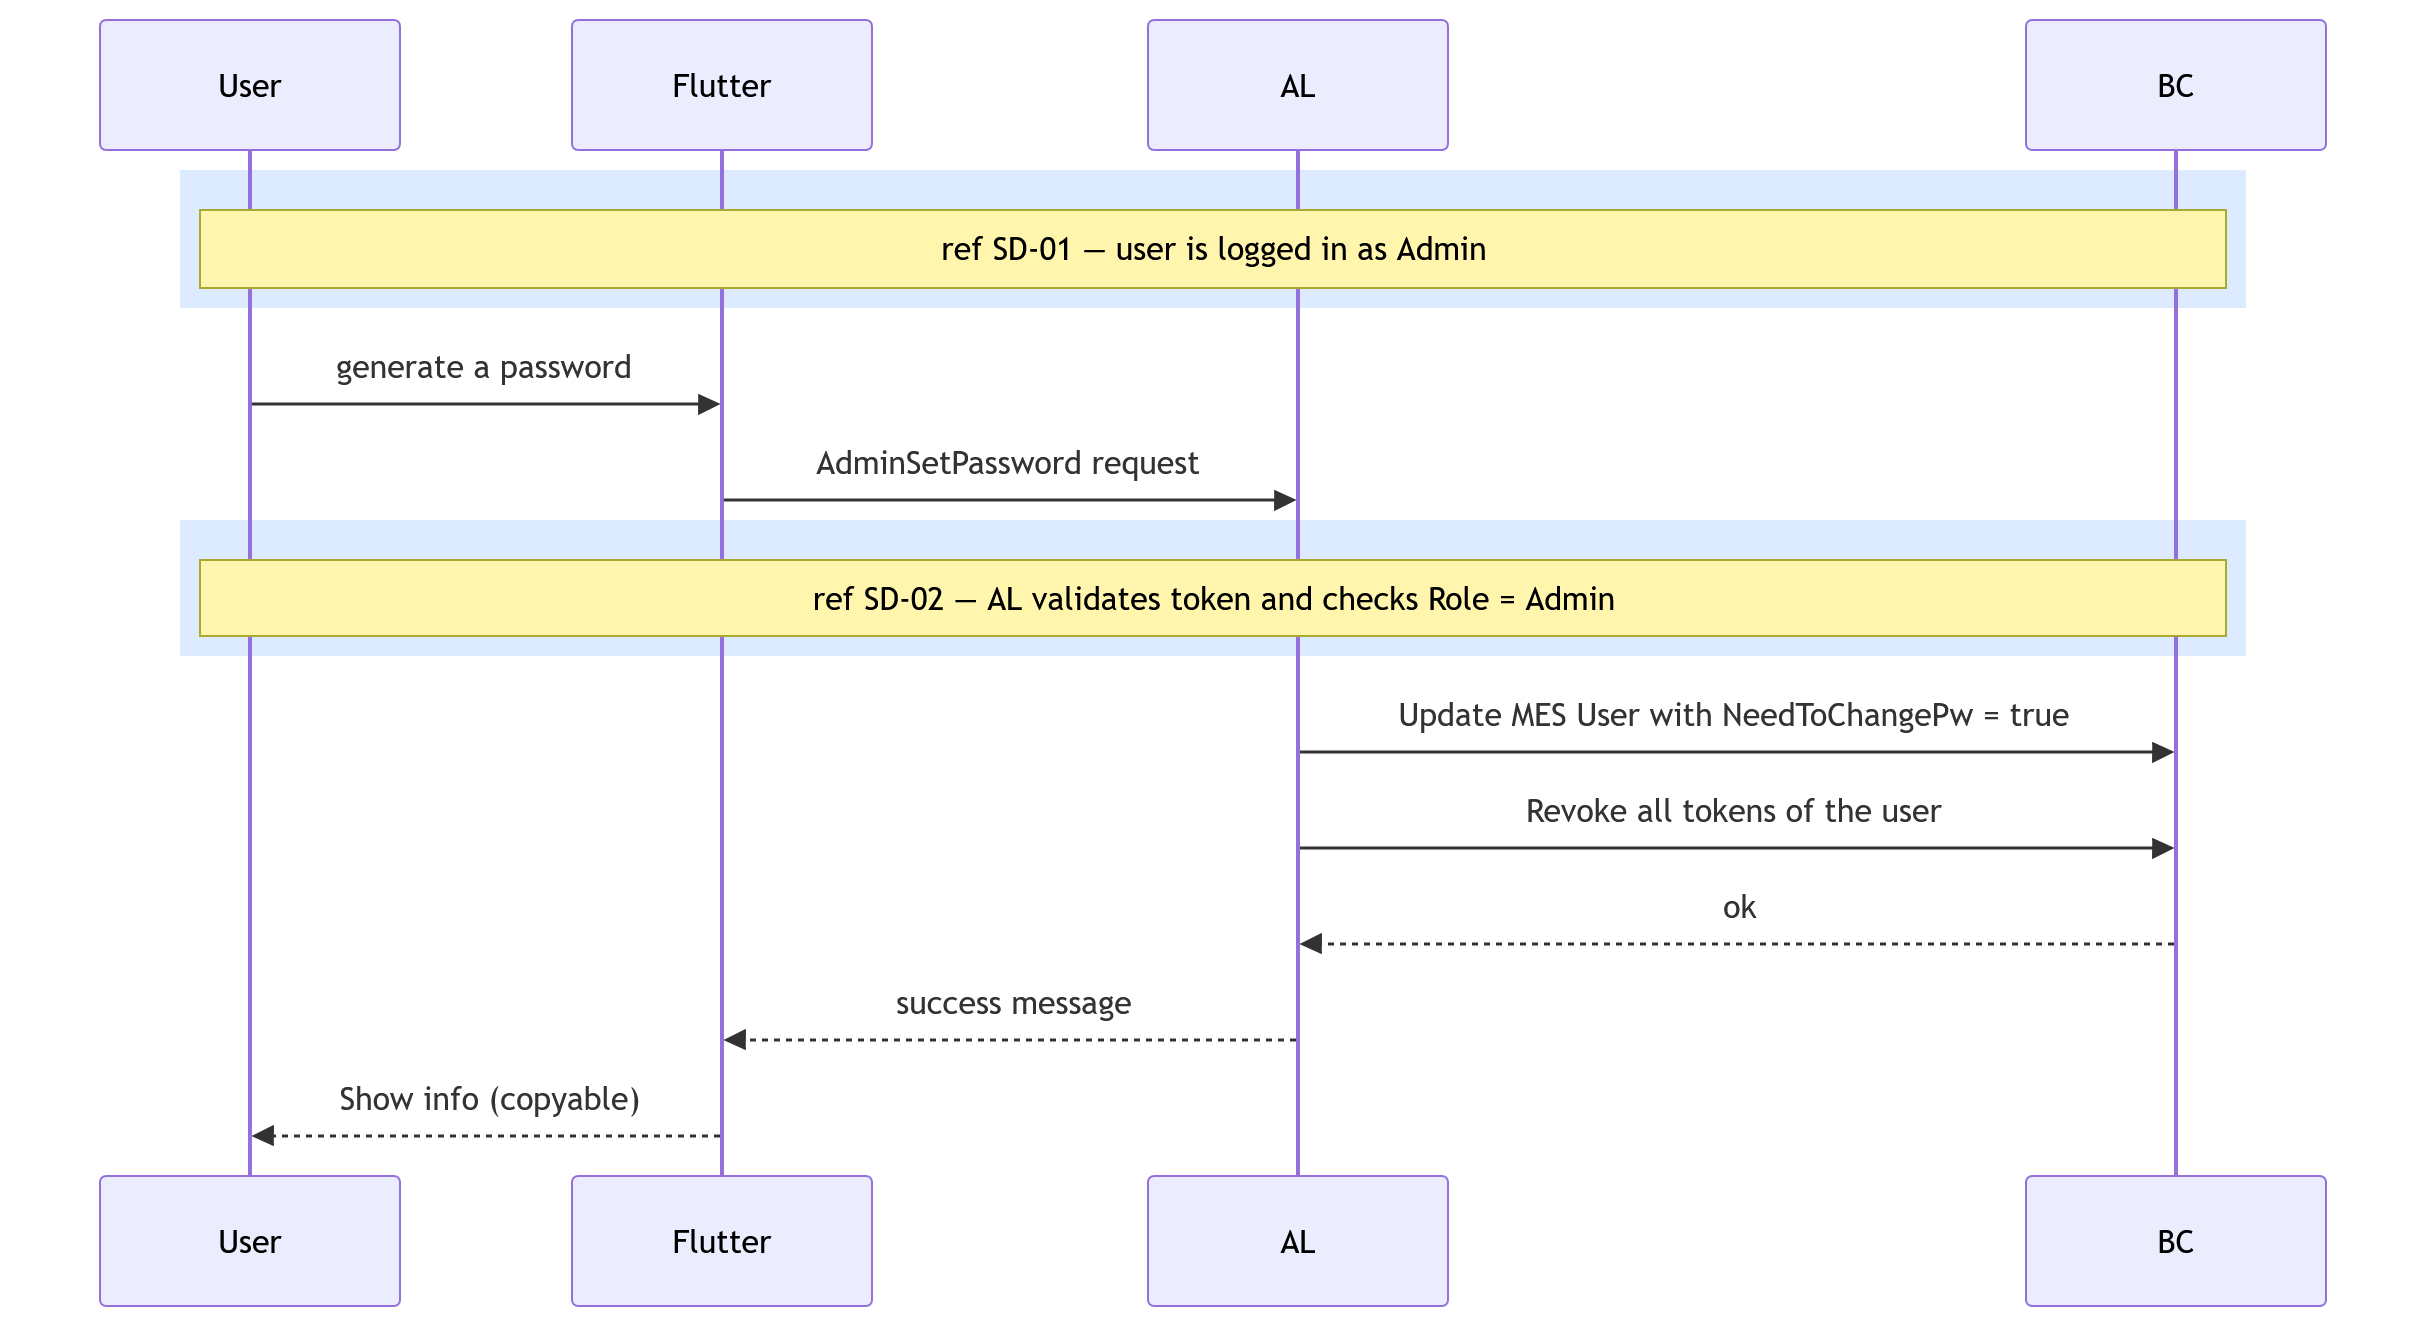
\includegraphics[width=\linewidth,height=0.82\textheight,keepaspectratio]{./media/MES_Sprint-1-Repport/diagrams/sequence/admin-set-password.png}%
	\caption{SD-06: Admin - Set Password.}%
	\label{fig:s1-seq-AdminSetPw}%
\end{figure}%


%=====SD-06==========================================================
% sequenceDiagram
%     actor User
%     participant Flutter
%     participant AL
%     participant BC

%     rect rgb(220,235,255)
%         Note over User,BC: ref SD-01 — user is logged in as Admin
%     end

%     User->>Flutter: generate a password
%     Flutter->>AL: AdminSetPassword request

%     rect rgb(220,235,255)
%         Note over User,BC: ref SD-02 — AL validates token and checks Role = Admin
%     end

%     AL->>BC: Update MES User with  NeedToChangePw = true
%     AL->>BC: Revoke all tokens of the user
%     BC-->>AL: ok
%     AL-->>Flutter: success message
%     Flutter-->>User: Show info (copyable)
%====================================================================

Figure~\ref{fig:s1-seq-AdminSetPw} depicts the admin set-password flow. The
administrator generates a temporary credential, the \techname{AL} layer marks
the target account as requiring a password change on next login, revokes all
active tokens for that account, and returns the new credential to the
\techname{Flutter} client as copyable text.

\begin{figure}[H]
	\centering
	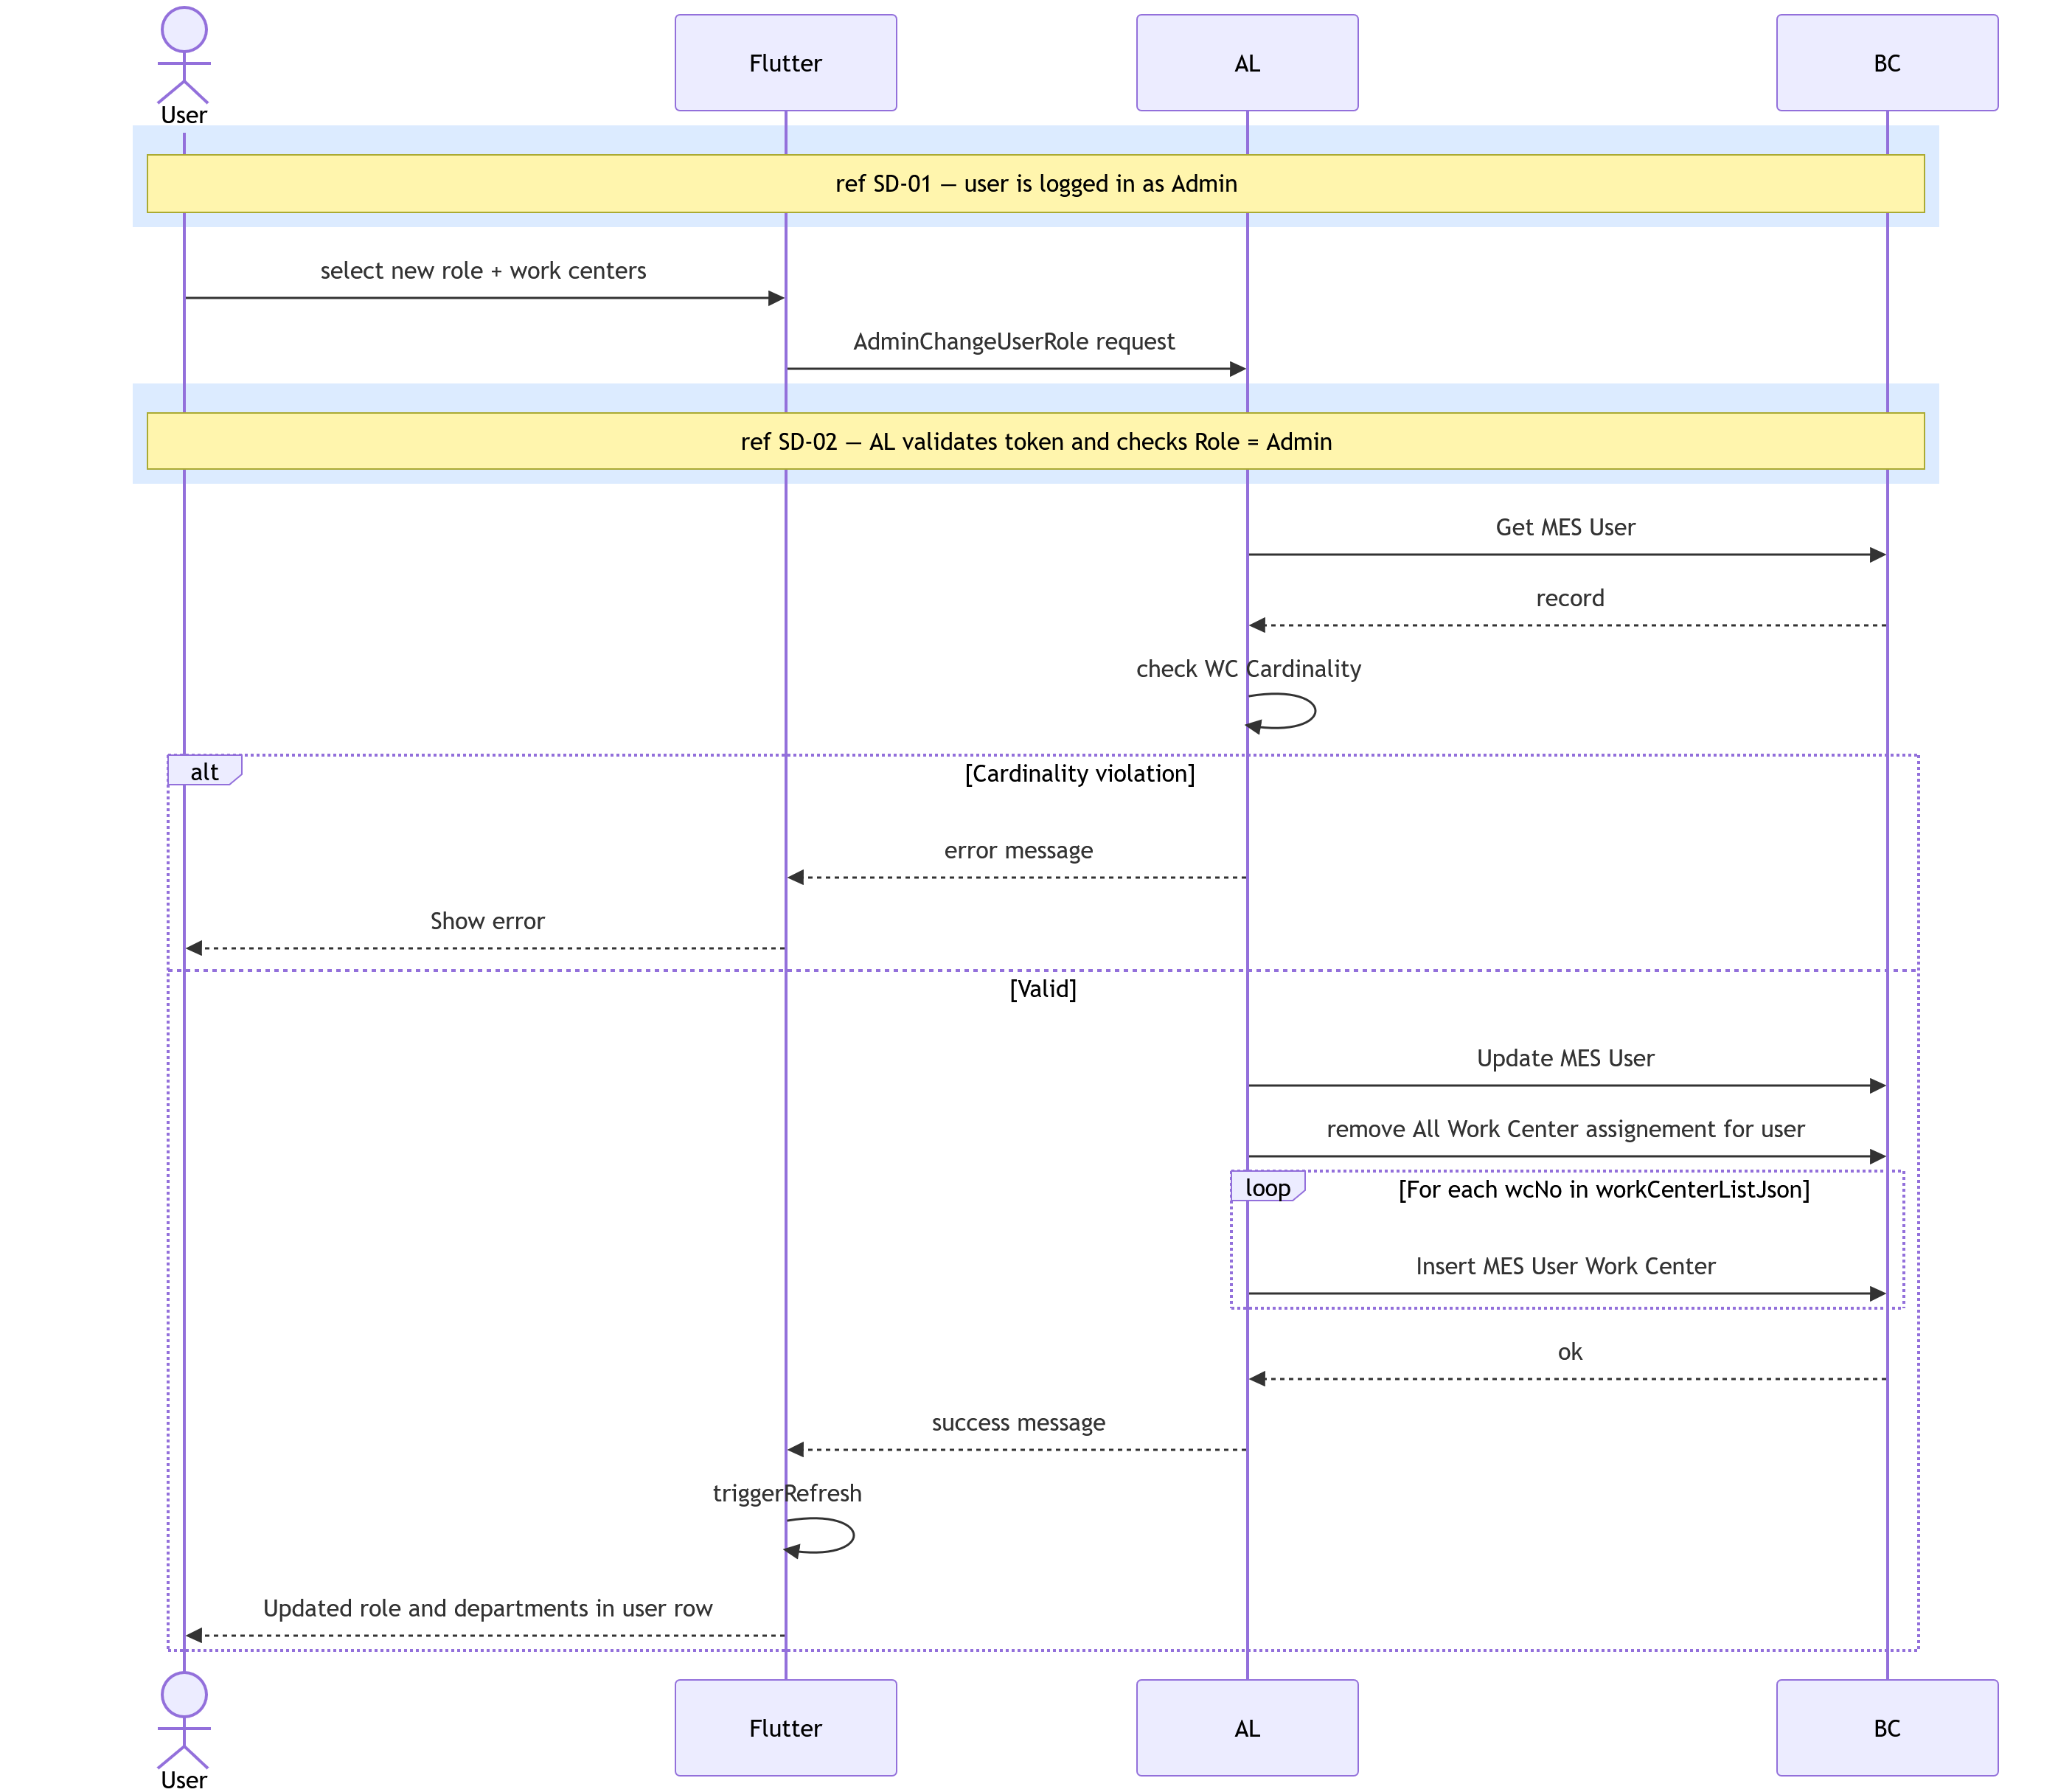
\includegraphics[width=\linewidth,height=0.82\textheight,keepaspectratio]{./media/MES_Sprint-1-Repport/diagrams/sequence/admin-change-role_departement.png}%
	\caption{SD-07: Admin - Change Role / Work Centre.}%
	\label{fig:s1-seq-AdminChangeRole}%
\end{figure}%

%=====SD-07===============================================================
% sequenceDiagram
%     actor User
%     participant Flutter
%     participant AL
%     participant BC

%     rect rgb(220,235,255)
%         Note over User,BC: ref SD-01 — user is logged in as Admin
%     end

%     User->>Flutter: select new role + work centers
%     Flutter->>AL: AdminChangeUserRole request

%     rect rgb(220,235,255)
%         Note over User,BC: ref SD-02 — AL validates token and checks Role = Admin
%     end

%     AL->>BC: Get MES User
%     BC-->>AL: record
%     AL->>AL: check WC Cardinality
%     alt Cardinality violation
%         AL-->>Flutter: error message
%         Flutter-->>User: Show error
%     else Valid
%         AL->>BC: Update MES User
%         AL->>BC: remove All Work Center assignement for user
%         loop For each wcNo in workCenterListJson
%             AL->>BC: Insert MES User Work Center
%         end
%         BC-->>AL: ok
%         AL-->>Flutter: success message
%         Flutter->>Flutter: triggerRefresh
%         Flutter-->>User: Updated role and departments in user row
%     end
%====================================================================

Figure~\ref{fig:s1-seq-AdminToggleActive} presents the account activation and
deactivation flow. When deactivating an account, the \techname{AL} layer
additionally revokes all active session tokens for that user, ensuring that
any currently authenticated sessions are immediately invalidated.

\begin{figure}[H]
	\centering
	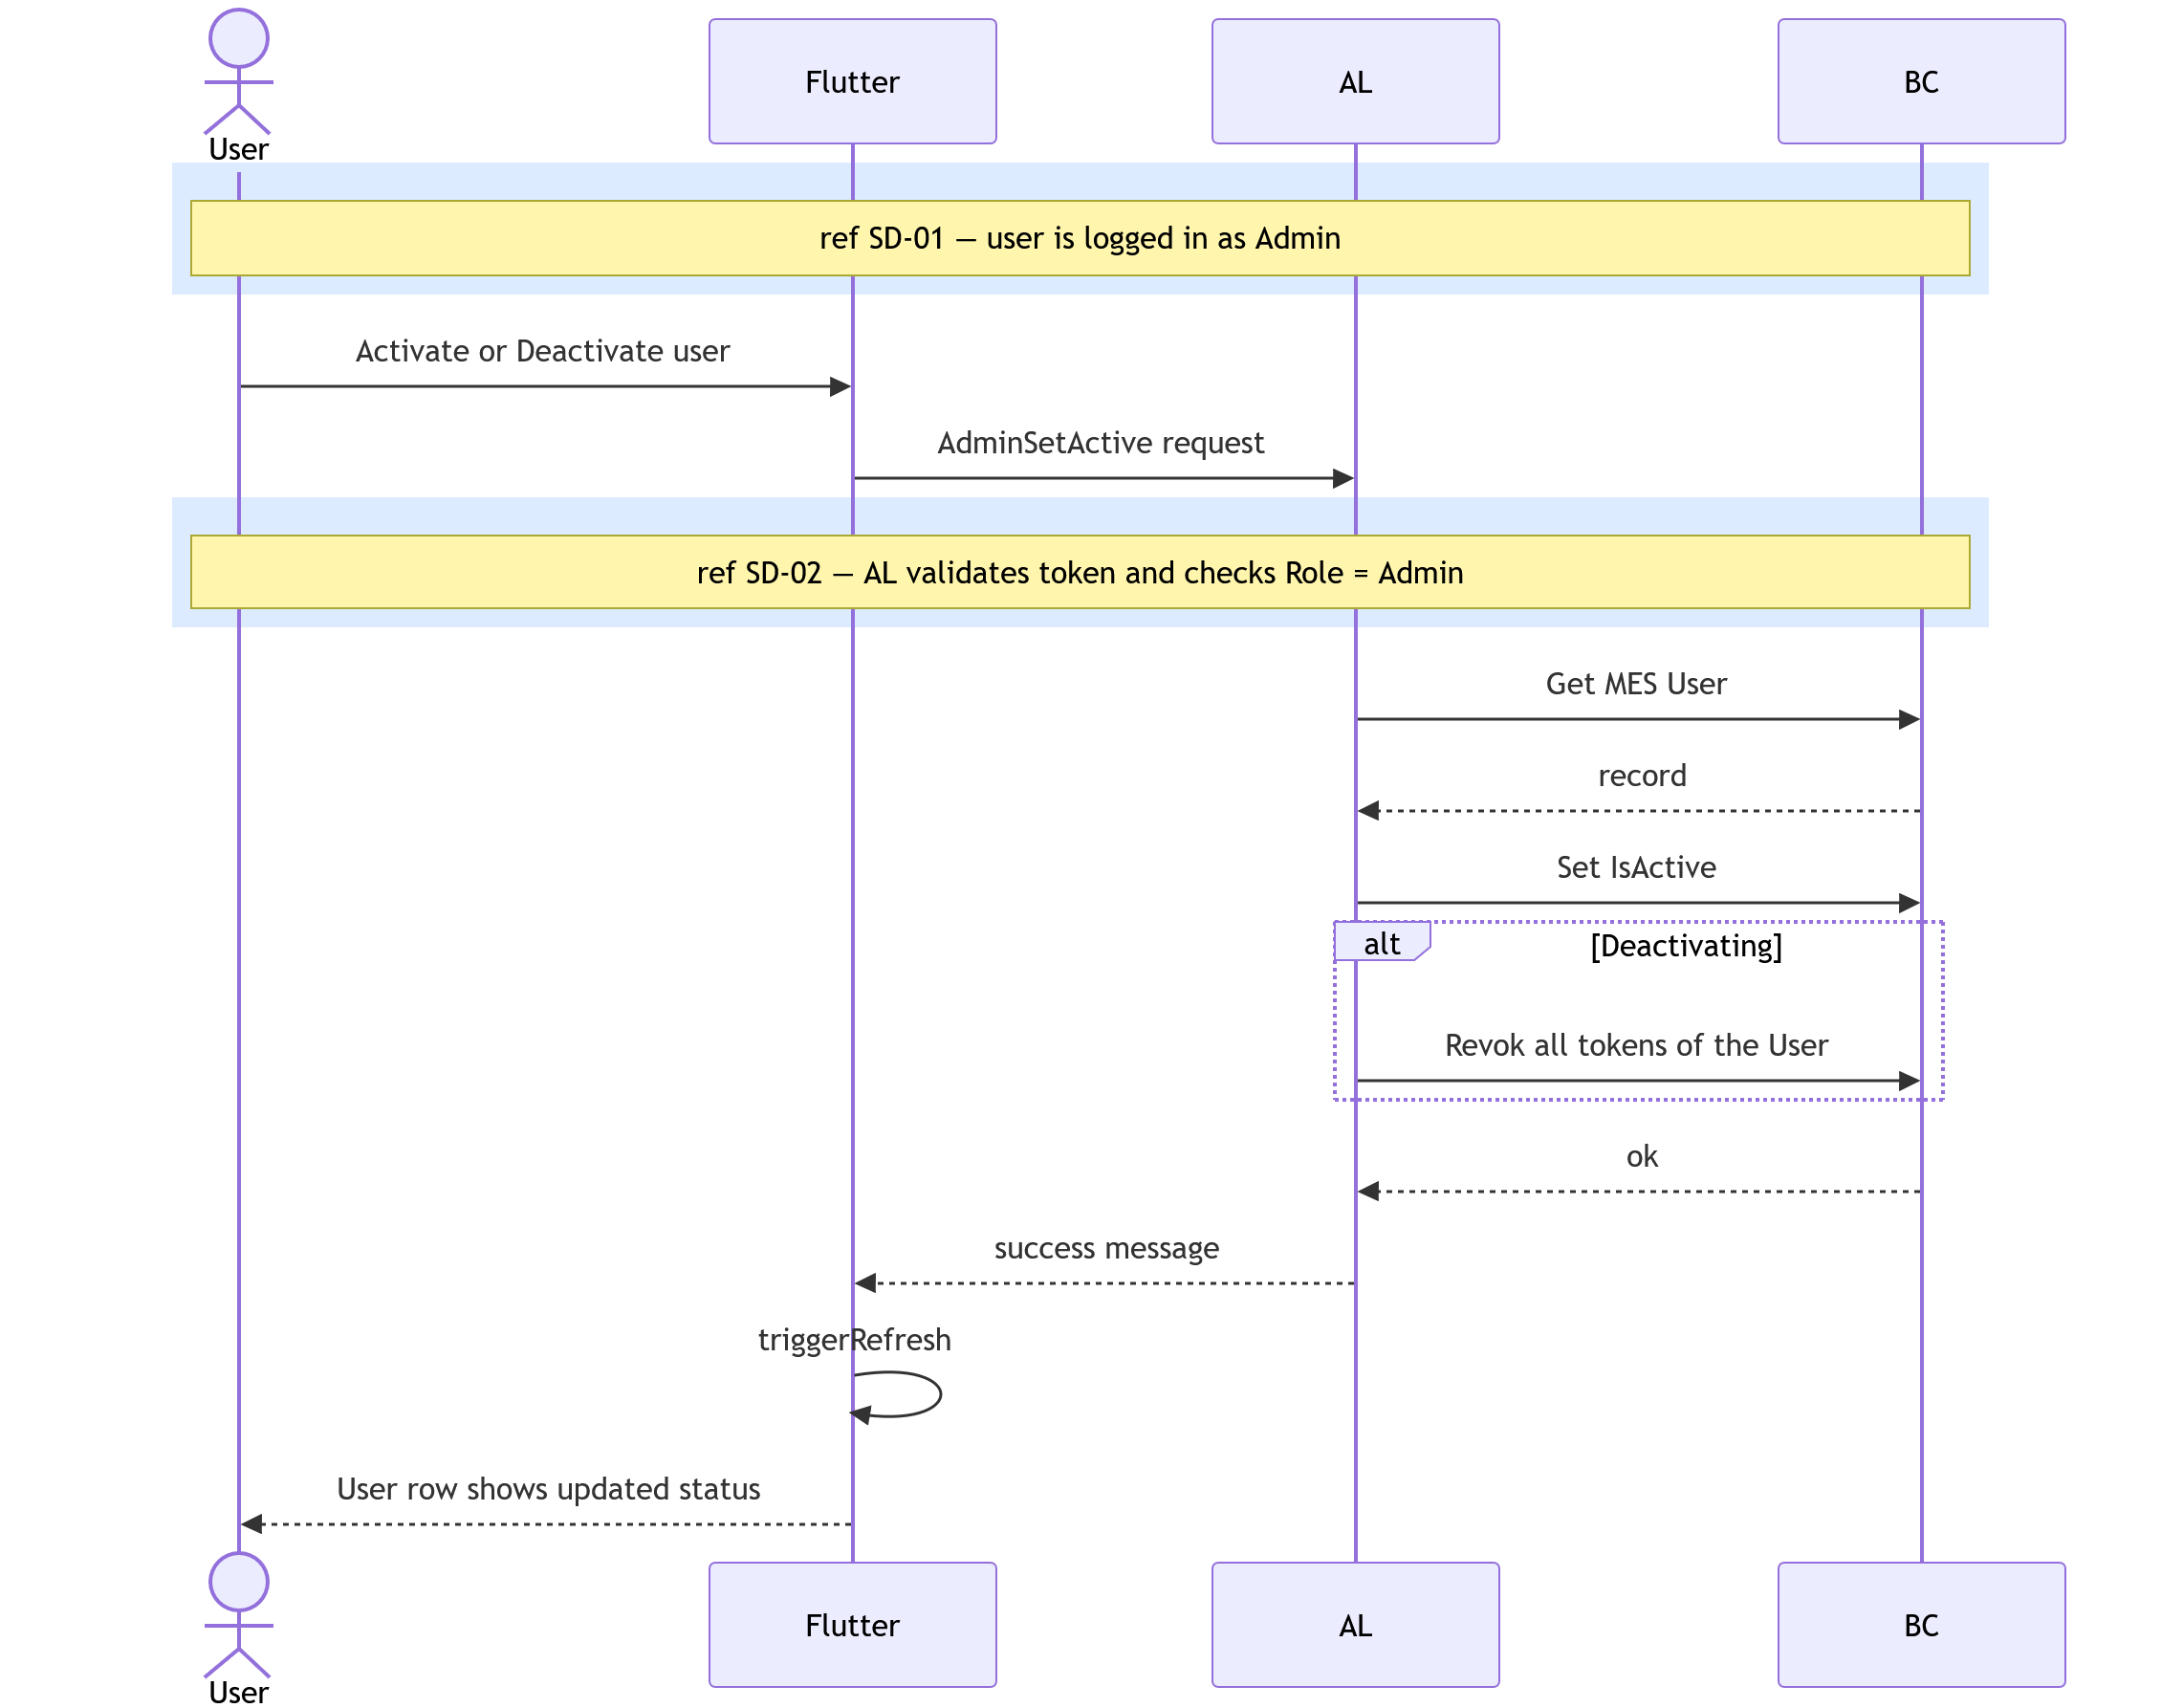
\includegraphics[width=\linewidth,height=0.82\textheight,keepaspectratio]{./media/MES_Sprint-1-Repport/diagrams/sequence/admin-toggle-account-active-status.png}%
	\caption{SD-08: Admin - Toggle Account Active Status.}%
	\label{fig:s1-seq-AdminToggleActive}%
\end{figure}%

%=====SD-08==========================================================
% sequenceDiagram
%     actor User
%     participant Flutter
%     participant AL
%     participant BC

%     rect rgb(220,235,255)
%         Note over User,BC: ref SD-01 — user is logged in as Admin
%     end

%     User->>Flutter: Activate or Deactivate user
%     Flutter->>AL: AdminSetActive request

%     rect rgb(220,235,255)
%         Note over User,BC: ref SD-02 — AL validates token and checks Role = Admin
%     end

%     AL->>BC: Get MES User
%     BC-->>AL: record
%     AL->>BC: Set IsActive
%     alt Deactivating
%         AL->>BC: Revok all tokens of the User
%     end
%     BC-->>AL: ok
%     AL-->>Flutter: success message
%     Flutter->>Flutter: triggerRefresh
%     Flutter-->>User: User row shows updated status
%====================================================================


\subsection{Class Diagram}

The UML Class Diagram of the \domainterm{MES} authentication domain, shown in
Figure~\ref{fig:s1-class-diagram}, depicts the \modulename{MesUser},
\modulename{AuthToken}, and \modulename{PasswordPolicy} classes with their
attributes and associations.

\begin{figure}[H]
	\centering
	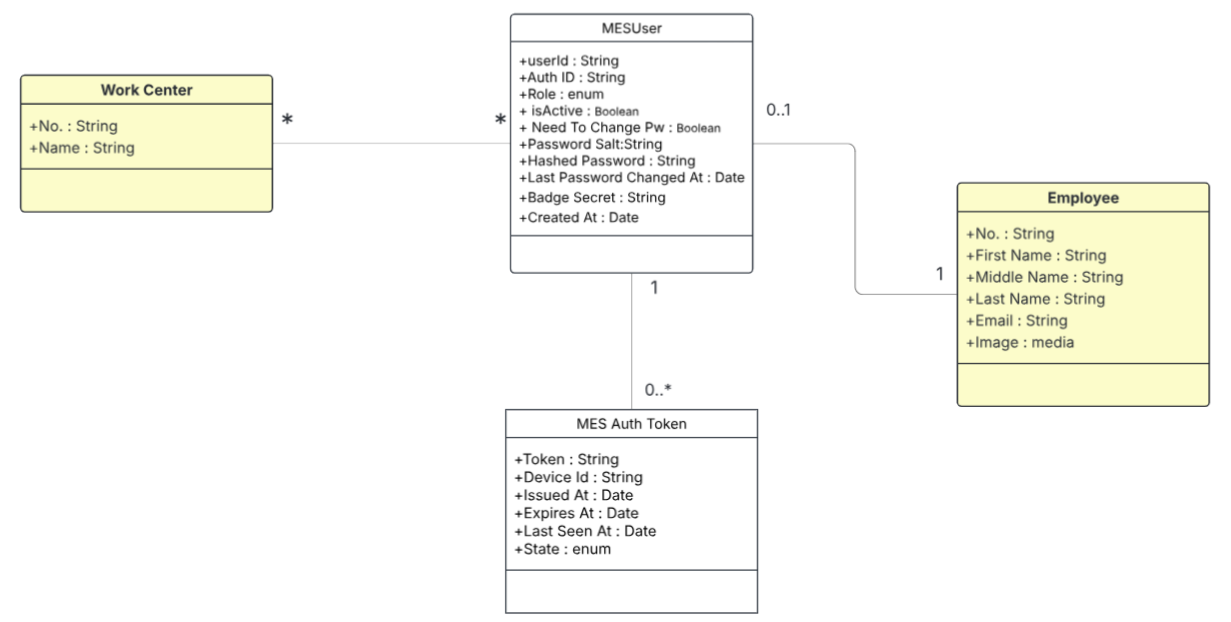
\includegraphics[width=\linewidth,keepaspectratio]{./media/MES_Sprint-1-Repport/diagrams/class/sprint1.png}
	\caption{UML Class Diagram.}
	\label{fig:s1-class-diagram}
\end{figure}


% -----------------------------------------------------------------------
\section{Implementation}
% -----------------------------------------------------------------------

\subsection{Backend Implementation}

\subsubsection{Backend Structure Overview}

The backend project structure is illustrated in Figure~\ref{fig:s1-backend-structure}.

\begin{figure}[H]
	\centering
	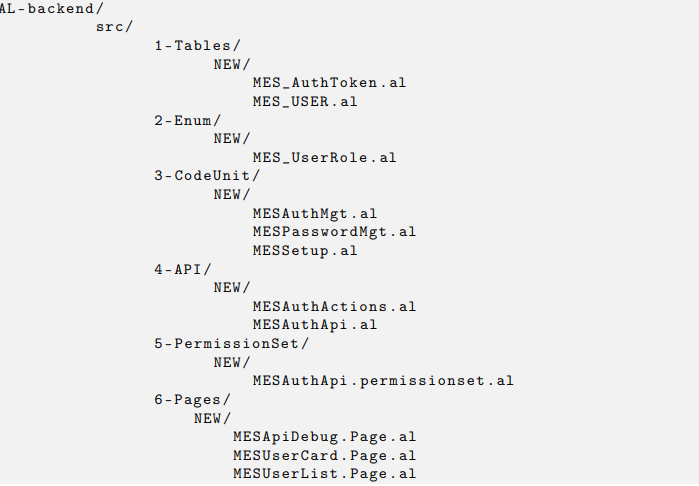
\includegraphics[width=\linewidth,keepaspectratio]{./media/MES_Sprint-1-Repport/image3.png}
	\caption{Backend project structure.}
	\label{fig:s1-backend-structure}
\end{figure}

\subsubsection{MES User Table Implementation}

The \modulename{MES User} table is implemented to store user information,
as described in Table~\ref{tab:s1-mes_user_fields}.

\begin{longtable}{@{} P{0.18\linewidth} P{0.18\linewidth} P{0.64\linewidth} @{}}
	
	\toprule
	\textbf{Name}     & \textbf{Type}                 & \textbf{Description} \\
	\midrule
	\endfirsthead
	
	\toprule
	\textbf{Name}     & \textbf{Type}                 & \textbf{Description} \\
	\midrule
	\endhead
	
	\multicolumn{3}{r}{\small Continued on next page} \\
	\endfoot
	
	\endlastfoot
	
	User Id           & Code[50]                      &                      
	Primary key. Login identifier used at the MES login prompt (e.g., \texttt{JDOE}, \texttt{OP001}). If blank on insert, a GUID-derived value is assigned automatically. \\
	\midrule
	
	Employee ID       & Code[50]                      &                      
	Foreign key to \texttt{Employee."No."}. Required for every MES account and enforced as unique (one Employee maps to one MES User). \\
	\midrule
	
	Auth ID           & Text[100]                     &                      
	Auto-generated external identifier in the form \texttt{AUTH-XXXXXXXX}. Used as the login identifier at the MES login prompt. Uniqueness enforced. \\
	\midrule
	
	Role              & Enum (\texttt{MES User Role}) &                      
	Authorization role for the MES application (e.g., Operator / Supervisor / Admin). Used to control permissions and access. \\
	\midrule
	
	%%% Work-centre assignments are stored in the separate MES User Work Center
	%%% junction table (Table 50115), not on MES User directly. Field removed. %%%
	%%%\midrule
	
	Is Active         & Boolean                       &                      
	Account enable/disable flag. If false, authentication is blocked and existing tokens are revoked when deactivated. \\
	\midrule
	
	Need To Change Pw & Boolean                       &                      
	If true, the user must change their password before using the MES application (set at creation and on forced password resets). \\
	\midrule
	
	Password Salt     & Text[64]                      &                      
	Random hex salt used in password hashing so identical passwords produce different hashes across users. \\
	\midrule
	
	Hashed Password   & Text[128]                     &                      
	Hashed password value (hex string). Passwords are never stored in plaintext; hashing uses the password plus salt. \\
	\midrule
	
	Created At        & DateTime                      &                      
	UTC timestamp set on insert only (audit trail/reporting). \\
	\midrule
	\noalign{\vskip 4pt}
	\caption{MES User (Table 50101) --- Field Dictionary}
	\label{tab:s1-mes_user_fields}
	
\end{longtable}

\subsubsection{Authentication Token Table}

The \modulename{MES Auth Token} table stores session information as described
in Table~\ref{tab:s1-mes_auth_token_fields}.

\begin{longtable}{@{} P{0.18\linewidth} P{0.18\linewidth} P{0.64\linewidth} @{}}
	
	\toprule
	\textbf{Name} & \textbf{Type} & \textbf{Description} \\
	\midrule
	\endfirsthead
	
	\toprule
	\textbf{Name} & \textbf{Type} & \textbf{Description} \\
	\midrule
	\endhead
	
	\multicolumn{3}{r}{\small Continued on next page} \\
	\endfoot
	
	\endlastfoot
	
	Token         & Guid          &                      
	Primary key. Raw GUID token presented by the client as a Bearer credential. Generated at issue time (never reused). Used for all direct token lookups (validation/logout). \\
	\midrule
	
	User Id       & Code[50]      &                      
	Foreign key to \texttt{MES User."User Id"}. Identifies the MES user who owns this session/token. Enforces referential integrity via \texttt{TableRelation}. \\
	\midrule
	
	Device Id     & Text[100]     &                      
	Optional identifier for the device that requested the token (e.g., \texttt{tablet-floor-02}, \texttt{scanner-01}). Stored for traceability/audit only; not used for validation. \\
	\midrule
	
	Issued At     & DateTime      &                      
	UTC timestamp set when the token is created. Useful for audit trail and token age inspection. \\
	\midrule
	
	Expires At    & DateTime      &                      
	UTC timestamp after which the token must be rejected even if not revoked. Set to \texttt{Issued At + TTL}. Token validation enforces \texttt{Expires At > CurrentDateTime()}. \\
	\midrule
	
	Last Seen At  & DateTime      &                      
	Updated on every successful token validation. Supports session monitoring (activity/idle detection). Not used for expiry enforcement (use \texttt{Expires At}). \\
	\midrule
	
	Revoked       & Boolean       &                      
	If true, token is explicitly invalidated and must be rejected even if not expired. Set on logout and during bulk revocation (e.g., password change, account deactivation). \\
	\midrule
	\noalign{\vskip 4pt}
	\caption{MES Auth Token (Table 50106) --- Field Dictionary}
	\label{tab:s1-mes_auth_token_fields}
	
\end{longtable}

Key points of the token design include a unique \domainterm{GUID} token,
auto-expiry after 12 hours, last activity tracking, and soft revocation.

\subsubsection{Password Management and Encryption}

The password management codeunit ensures that plaintext is never persisted. A
unique random \domainterm{salt} (64-character SHA-256 hex string) is generated per
user and the password is hashed using single-pass \domainterm{SHA-256} before storage.
Data classification attributes mark sensitive fields as \emph{Customer Content}
or \emph{System Metadata}.

Key points include: passwords are never stored in plaintext; a unique salt per user
(64 characters) is generated; \domainterm{SHA-256} hashing is applied; and data is
classified as \emph{Customer Content} or \emph{System Metadata}.

\subsubsection{Authentication Logic --- Login, Logout, and Change Password}

\textbf{Login}

The login validates the user credentials against the \modulename{MES User}
table. If the credentials are correct and the account is active, a token will
be generated and stored in the \modulename{MES Auth Token} table.

The system returns a \domainterm{JSON} login response object which includes the
generated session token, the authenticated user's role string, and a boolean
\domainterm{needChangePassword} flag consumed by the \techname{Flutter} frontend
to decide the post-login navigation target.

\textbf{Logout}

On logout, the user's session authentication token is revoked. The token
record matching the supplied session token is located in the
\modulename{MES Auth Token} table and its \texttt{Revoked} flag is set to
\texttt{true}, immediately invalidating the session (soft revocation).

\textbf{Change Password}

Changing password requires a valid authentication token, a correct current
password, and a new password that complies with security rules.

\subsection{REST API and Web Services Implementation}

To enable communication between \techname{Flutter} and
\techname{Microsoft Dynamics Business Central}, a set of \domainterm{RESTful APIs}
were implemented using AL.

\subsubsection{API Pages for MES User Management}

The \domainterm{API Page} definition for the \apiendpoint{/mesUsers} endpoint
exposes the \modulename{MES User} table as a read-only \domainterm{OData} feed.

The \domainterm{API Page} definition for the \apiendpoint{/createMesUser}
endpoint differs from the read endpoint by setting validation triggers.
\texttt{DelayedInsert\,=\,true} buffers all field values until the
complete request body has been received before committing the new
\modulename{MES User} record to the database.

Key point: the difference between these two APIs is the \domainterm{Delayed Insert} flag.
When set to \texttt{true}, it delays insertion until all fields are received,
which is required for \texttt{POST} operations. \texttt{GET} is not affected.

\subsubsection{OData Functions and Web Service Configuration}

Built \techname{MESUnboundActions} codeunit (50125): \texttt{Login()}, \texttt{Logout()}, \texttt{Me()}, \texttt{ChangePassword()}.
Exposed these functions in the \techname{MES Web Service} codeunit (50126) exposed via ODataV4.
Configured \techname{WebServices.xml} to publish \techname{MES Web Service}
(codeunit 50126) as an ODataV4 web service under the service name
\texttt{MESWebService}.

\subsection{Frontend Implementation}

The frontend of this system was developed using \techname{Flutter}. The
application is structured into four main layers: a \textbf{\domainterm{UI Layer}}
consisting of Screens and Widgets; a \textbf{\domainterm{State Management Layer}}
built on Providers; a \textbf{\domainterm{Service Layer}} for API communication;
and a \textbf{\domainterm{Model Layer}} for Data Models.


\noindent
\begin{minipage}[t]{0.6\textwidth}
	The data flow follows a unidirectional pattern from the \domainterm{UI Layer}
	through the \domainterm{State Management Layer} (\modulename{Provider} pattern)
	and \domainterm{Service Layer} to the \techname{Business Central} REST API backend,
	as illustrated in Figure~\ref{fig:s1-flutter-architecture-s1}.
	\subsubsection{Service Layer (API Communication)}

	The \domainterm{Service Layer} is responsible for handling all \domainterm{HTTP}
	communication between \techname{Flutter} and the \techname{Business Central} backend.

	Two services were implemented: the \modulename{api\_service} manages
	authentication requests such as \uilabel{login}, \uilabel{logout}, and
	\uilabel{password change}, while the \modulename{mes\_user\_service} handles MES
	user operations including fetching and creating new users.

	\textbf{\modulename{api\_service.dart}}

	The class declaration and constructor show the base URL configuration and
	\domainterm{HTTP} client initialisation used by all authentication endpoints.
	The \uilabel{login} method sends user credentials and device ID to the \apiendpoint{/login} endpoint and parses the returned session token, role, and \domainterm{needChangePassword} flag. The \uilabel{logout} method sends the active session token to the \apiendpoint{/logout} endpoint to trigger server-side token revocation.

\end{minipage}
\hfill
\begin{minipage}[t]{0.38\textwidth}
  \vspace{0pt}
  \centering
  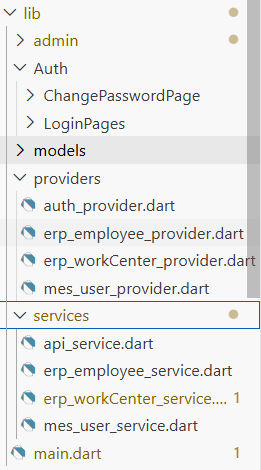
\includegraphics[width=\linewidth,keepaspectratio]{./media/MES_Sprint-1-Repport/image13.png}
  \captionof{figure}{\techname{Flutter} layered architecture.}
  \label{fig:s1-flutter-architecture-s1}
\end{minipage}

The \uilabel{change password} method submits the current password,
new password, and session token to the \apiendpoint{/changePassword} endpoint.
Shared error-handling and response-parsing utilities are used by all methods in
the service class to propagate structured exceptions to the
\domainterm{State Management Layer}.

\textbf{\modulename{mes\_user\_service.dart}}

The class declaration and \uilabel{fetch users} method send an authenticated
\domainterm{HTTP GET} request to the \apiendpoint{/mesUsers} endpoint and
deserialise the response into a list of \modulename{MesUser} model objects.
The \uilabel{create user} method sends a \domainterm{HTTP POST} request to the
\apiendpoint{/createMesUser} endpoint with the new user's role and employee
reference in the request body. The \uilabel{generate password} method and
associated response deserialisers handle the password generation endpoint and
map the \domainterm{JSON} result into the \modulename{GeneratedPassword} model.

\subsubsection{State Management Layer using Provider}

The \domainterm{Provider} pattern is implemented to ensure reactive UI updates
and centralised data handling. Two providers were implemented:
\modulename{AuthProvider}, which manages authentication state, and
\modulename{MesUserProvider}, which handles MES user data. Each provider wraps
the corresponding service layer calls and exposes reactive state (authenticated
user, user list, loading flag, error message) consumed by the \domainterm{UI Layer}
via \texttt{context.watch}.

\subsubsection{User Interface}

The \uilabel{Login Page}, shown in Figure~\ref{fig:s1-ui-login}, is the application
entry screen presented to all users on launch. It contains \uilabel{User ID} and
\uilabel{Password} input fields and a \uilabel{Login} button. Successful
authentication redirects the user to the role-appropriate dashboard.

\begin{figure}[H]
	\centering
	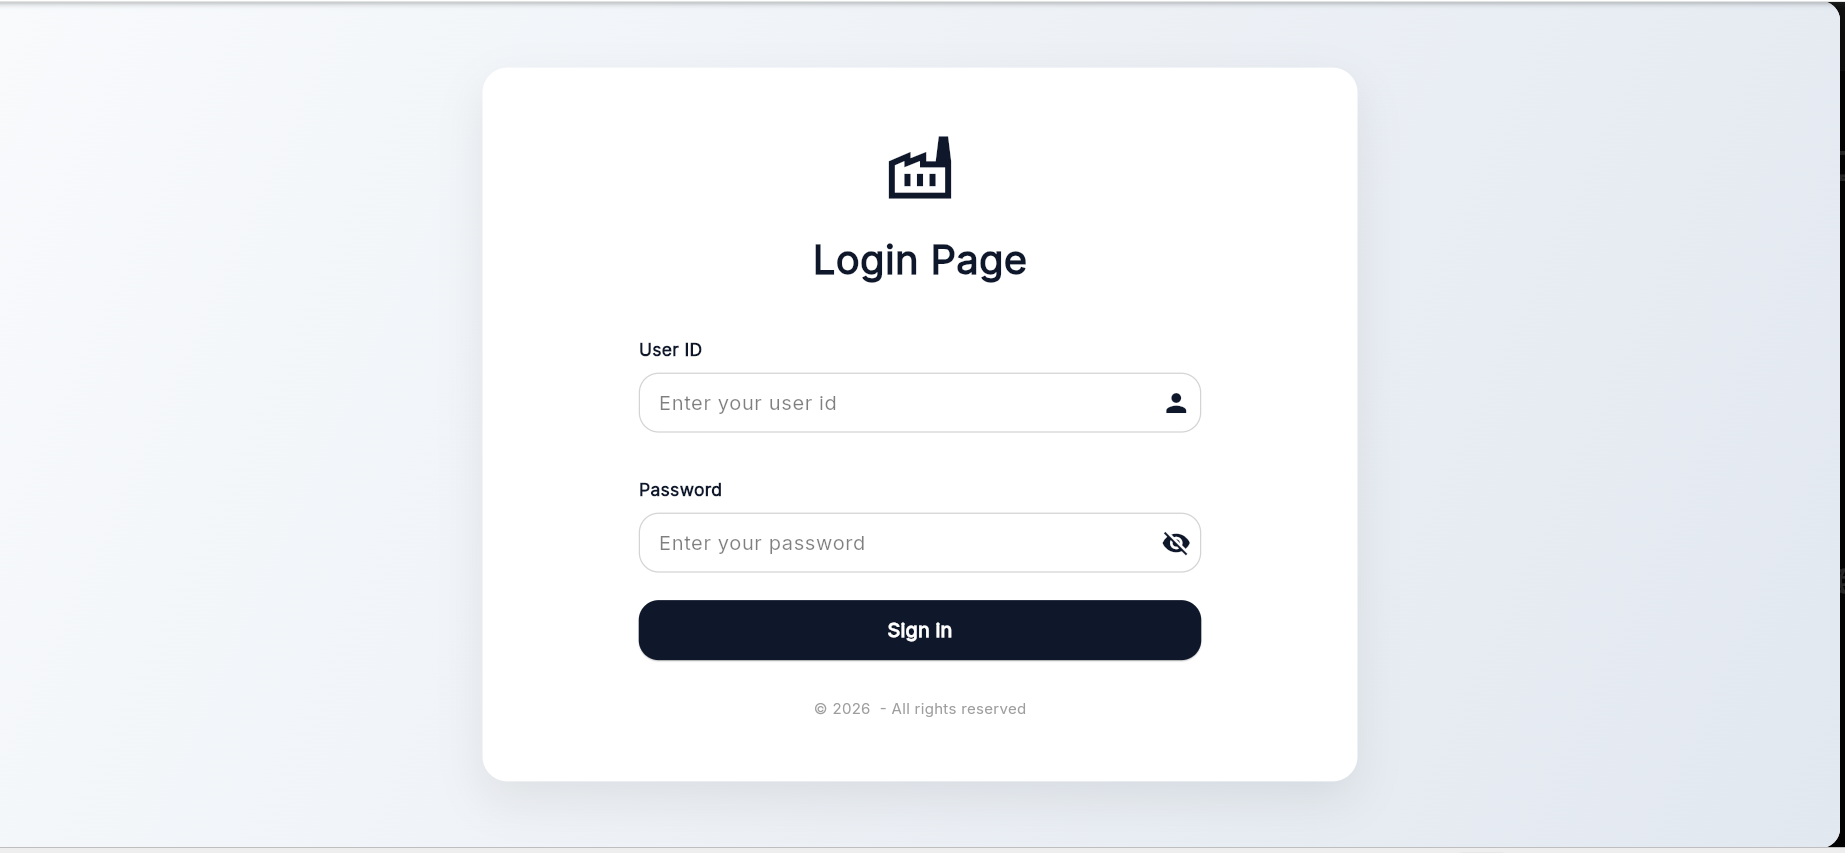
\includegraphics[width=\linewidth,keepaspectratio]{./media/MES_Sprint-1-Repport/image23.png}
	\caption{\uilabel{Login Page}.}
	\label{fig:s1-ui-login}
\end{figure}

The \uilabel{MES User List Page}, shown in Figure~\ref{fig:s1-ui-user-list}, is
the \userrole{Administrator} dashboard screen listing all registered
\domainterm{MES} users with their assigned roles and active status, providing
action buttons to assign roles or generate passwords for each employee.

\begin{figure}[H]
	\centering
	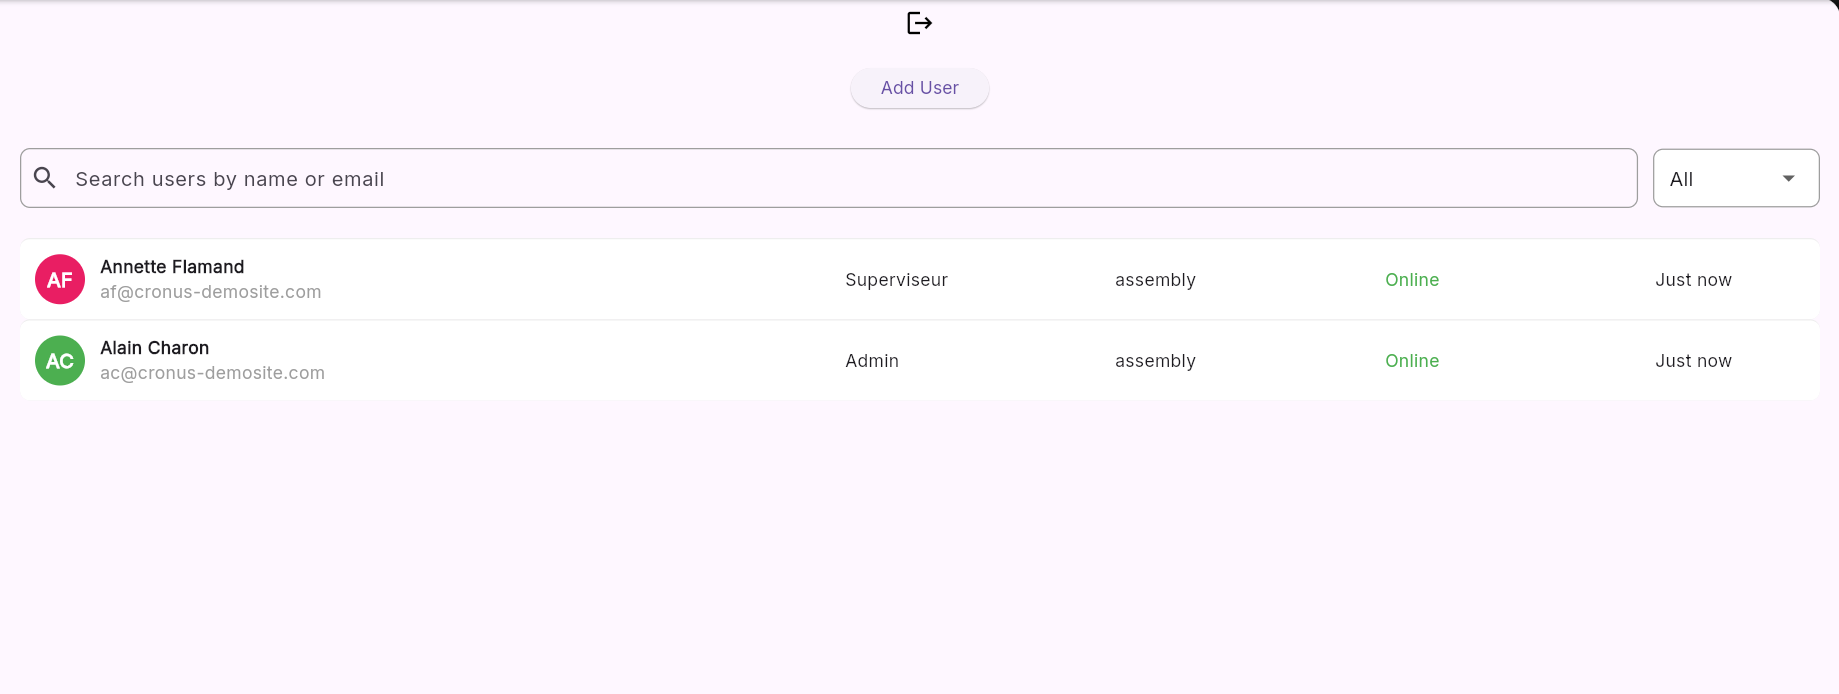
\includegraphics[width=\linewidth,keepaspectratio]{./media/MES_Sprint-1-Repport/image24.png}
	\caption{\uilabel{MES User List Page}.}
	\label{fig:s1-ui-user-list}
\end{figure}

The \uilabel{Assign MES Role Dialog}, shown in Figure~\ref{fig:s1-ui-assign-role},
is a modal dialog allowing the \userrole{Administrator} to select a
\techname{Business Central} employee record and assign them an \domainterm{MES}
role (\userrole{Operator} or \userrole{Supervisor}), creating a new
\modulename{MES User} record via the \apiendpoint{/createMesUser} endpoint.

\begin{figure}[H]
	\centering
	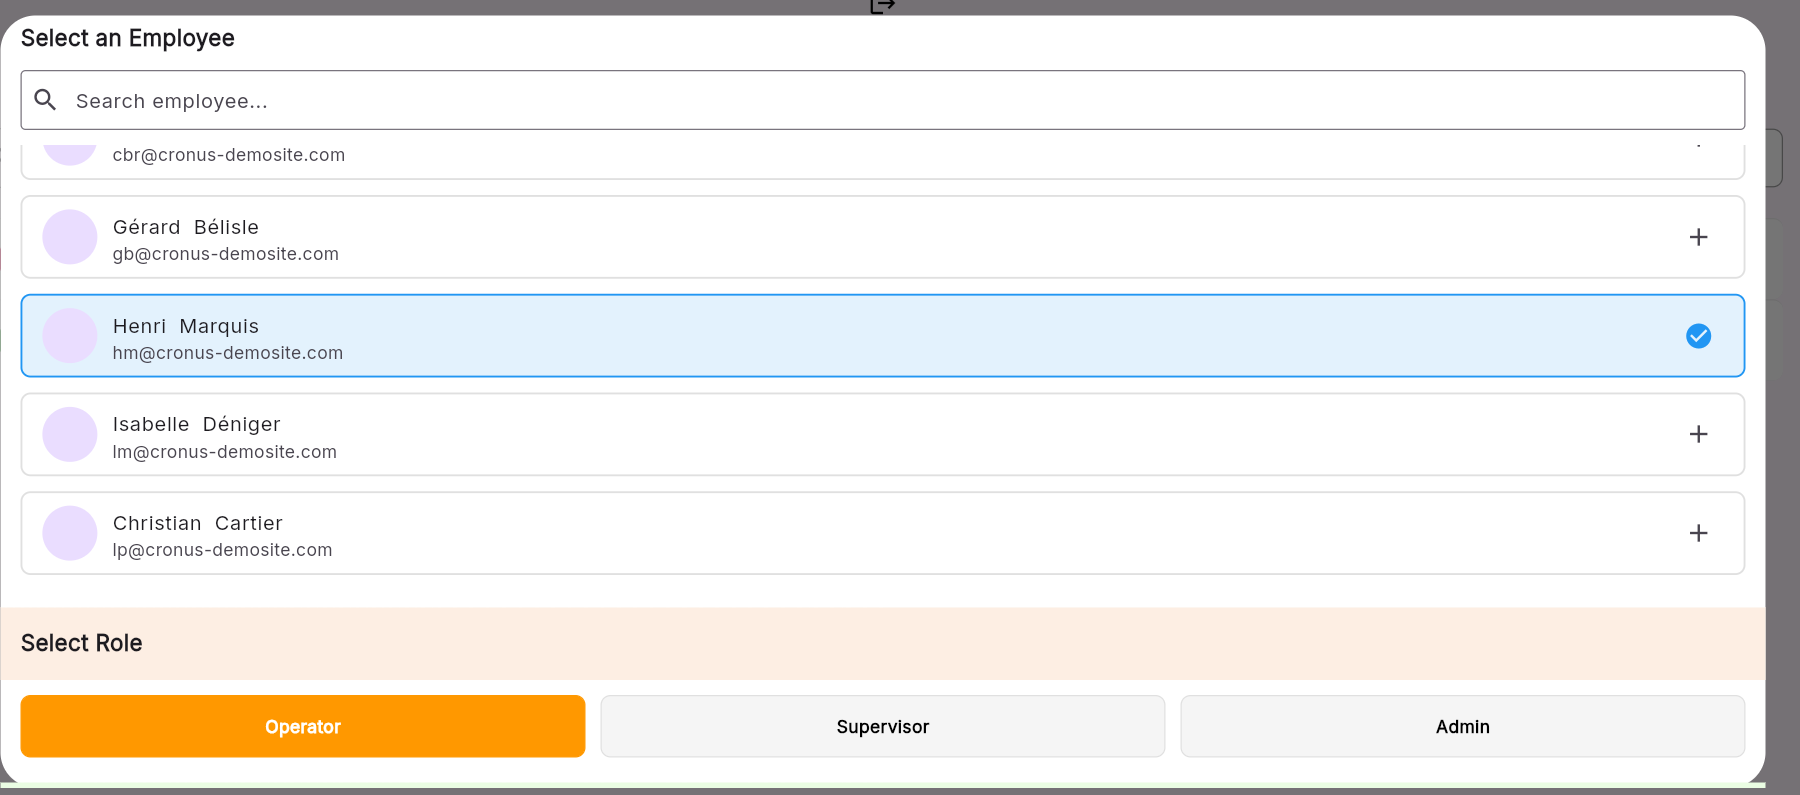
\includegraphics[width=\linewidth,keepaspectratio]{./media/MES_Sprint-1-Repport/image25.png}
	\caption{\uilabel{Assign MES Role Dialog}.}
	\label{fig:s1-ui-assign-role}
\end{figure}

The \uilabel{Generate Password Dialog}, shown in Figure~\ref{fig:s1-ui-generate-password},
is a modal dialog through which the \userrole{Administrator} triggers server-side
secure password generation for a selected \domainterm{MES} user. The generated
password is displayed once and must be communicated to the user out-of-band.

\begin{figure}[H]
	\centering
	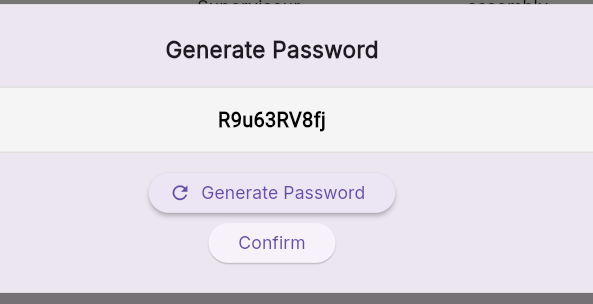
\includegraphics[width=\linewidth,keepaspectratio]{./media/MES_Sprint-1-Repport/image26.png}
	\caption{\uilabel{Generate Password Dialog}.}
	\label{fig:s1-ui-generate-password}
\end{figure}

The \uilabel{Password Generated Successfully Dialog}, shown in
Figure~\ref{fig:s1-ui-password-success}, is a confirmation dialog showing the
plaintext password to the \userrole{Administrator} for one-time transmission to
the user. The password is not stored in plaintext on the server after this point.

\begin{figure}[H]
	\centering
	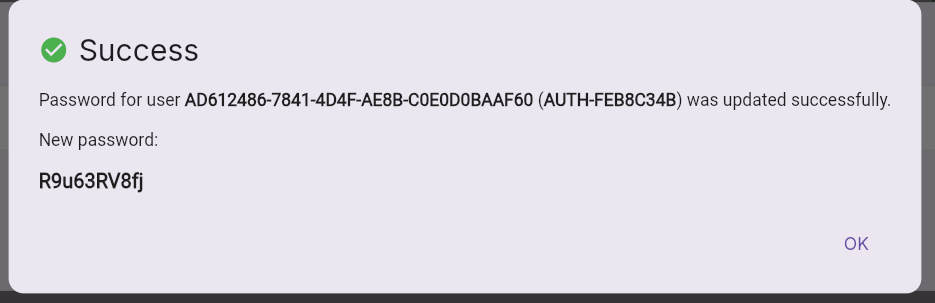
\includegraphics[width=\linewidth,keepaspectratio]{./media/MES_Sprint-1-Repport/image27.png}
	\caption{\uilabel{Password Generated Successfully Dialog}.}
	\label{fig:s1-ui-password-success}
\end{figure}

The \uilabel{Change Password Page}, shown in Figure~\ref{fig:s1-ui-change-password},
is presented to users whose \domainterm{needChangePassword} flag is \texttt{true}
after login, requiring them to enter their current password and choose a new
password before accessing the main application.

\begin{figure}[H]
	\centering
	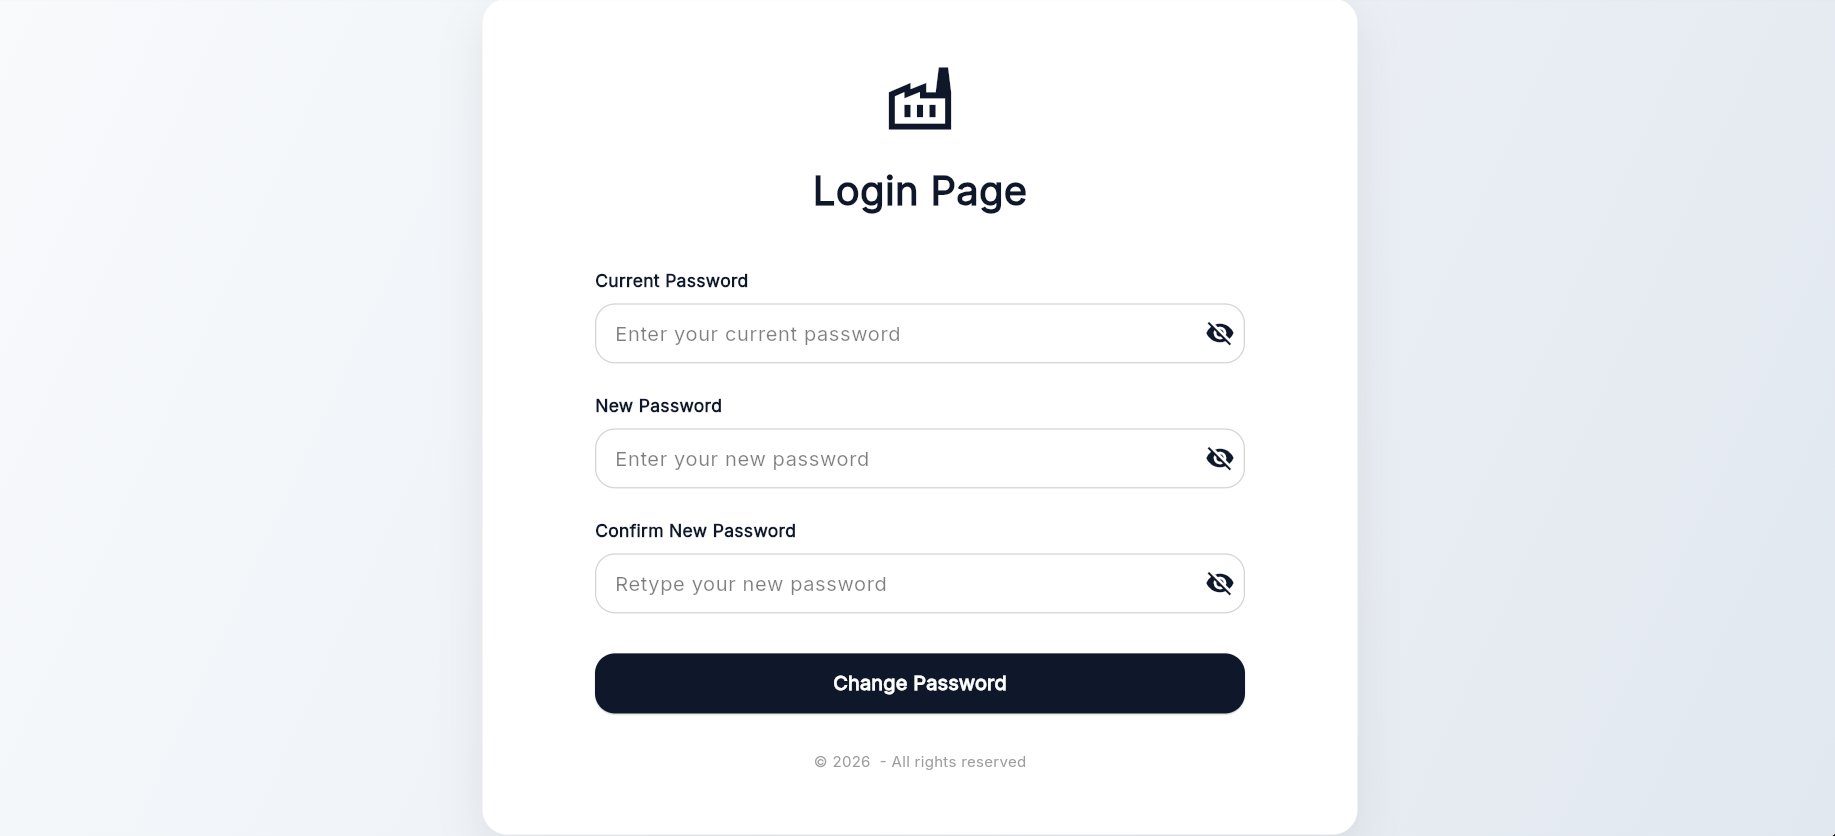
\includegraphics[width=\linewidth,keepaspectratio]{./media/MES_Sprint-1-Repport/image28.png}
	\caption{\uilabel{Change Password Page}.}
	\label{fig:s1-ui-change-password}
\end{figure}

The \uilabel{Change Role Dialog}, shown in Figure~\ref{fig:s1-ui-chRole-diag},
is a modal dialog through which the \userrole{Administrator} updates the
role and work-centre assignment of an existing \domainterm{MES} user. The
dialog pre-populates the current role and presents a three-button row
(Operator / Supervisor / Admin); selecting Admin hides the work-centre list,
selecting Operator shows a single-select list, and selecting Supervisor shows
a multi-select list. An inline error banner displays any server-side validation
failure. Tapping \uilabel{Save Changes} submits the update and revokes all
active tokens for the affected user.

\begin{figure}[H]
	\centering
	
\includegraphics[width=\linewidth,keepaspectratio]{./media/MES_Sprint-1-Repport/placeholder-image.png}
	\caption{\uilabel{Change Role Dialog}.}
	\label{fig:s1-ui-chRole-diag}
\end{figure}

The user row in the \uilabel{MES User List Page} now includes a
\texttt{PopupMenuButton} action menu accessible via a trailing icon on each row.
The menu exposes two actions: \uilabel{Change Role / Department}, which opens the
\techname{ChangeRoleDialog} described above, and \uilabel{Activate} or
\uilabel{Deactivate}, whose label switches dynamically based on the user's current
\texttt{isActive} flag. Selecting \uilabel{Deactivate} immediately revokes all
active sessions for that account; selecting \uilabel{Activate} re-enables login.

\section{Testing and Validation}
\subsection{Integration testing}
For integration testing, we chose Postman, a powerful and user-friendly tool for API evaluation. Figure~\ref{fig:s1-test-postman-fetchAllMesUsers} shows a test case for the \apiendpoint{/mesUsers} endpoint.

\begin{figure}[H]
	\centering
	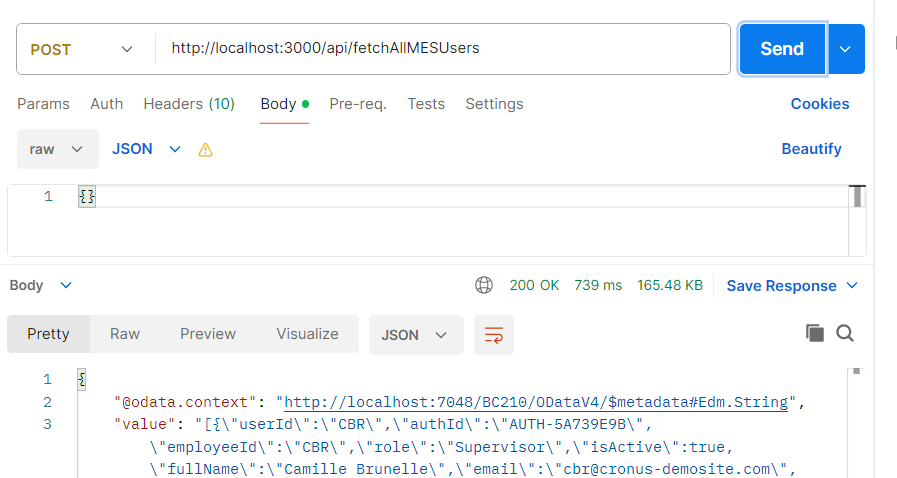
\includegraphics[width=\linewidth,keepaspectratio]{./media/MES_Sprint-1-Repport/tests/postman/fetchAllMesUsers.png}
	\caption{Postman endpoint test --- fetchAllMesUsers.}
	\label{fig:s1-test-postman-fetchAllMesUsers}
\end{figure}


% -----------------------------------------------------------------------
\phantomsection
\section*{Conclusion}
\addcontentsline{toc}{section}{Conclusion}
% -----------------------------------------------------------------------

This sprint successfully delivered a complete authentication and user management
foundation for the \domainterm{MES} application. The backend, built in
\techname{Microsoft Dynamics Business Central} using \techname{AL}, implements
secure credential validation, \domainterm{SHA-256} password hashing,
session token management with automatic expiry, and a full set of
\domainterm{RESTful} API endpoints exposed through \techname{MES Web Service}
(codeunit 50126). The \techname{Flutter} frontend provides a clean, role-aware
user experience covering login, logout, forced password change, administrator-level
user creation, role and work-centre management, and account activation control.
